\documentclass[lettersize,journal]{IEEEtran}

% \PassOptionsToPackage{table}{xcolor}
\usepackage{microtype}
\usepackage{flushend}
\usepackage{enumitem}
\usepackage{booktabs}
\usepackage{hyperref}
\usepackage{tikz}
\usepackage{color, colortbl}
\usepackage{makecell}
\usepackage{multirow}
% \usepackage[table]{xcolor}
\usepackage{xstring}
\usepackage{amsmath}

\usepackage{pifont}
\newcommand{\tick}{\ding{51}}%
\newcommand{\cross}{\ding{55}}%
\usepackage{makecell}
\usepackage{textcomp}
\usepackage[normalem]{ulem}
\usepackage{array}
\usepackage{textcomp}
\usepackage{url}
\usepackage{stfloats}
\usepackage{verbatim}
\usepackage{graphicx}
\usepackage{cite}


\usepackage[caption=false,font=normalsize,labelfont=sf,textfont=sf]{subfig}
\hyphenation{op-tical net-works semi-conduc-tor IEEE-Xplore}
\hypersetup{
colorlinks=true,
linkcolor=black
}
\hypersetup{hidelinks} 

\usetikzlibrary{fit,calc}
%define a marking command
\newcommand*{\tikzmk}[1]{\tikz[remember picture,overlay,] \node (#1) {};\ignorespaces}
%define a boxing command, argument = colour of box
\newcommand{\boxit}[1]{\tikz[remember picture,overlay]{\node[xshift=-15pt,yshift=0.5pt,fill=#1,opacity=.25,fit={(A)($(B)+(.9\linewidth,.8\baselineskip)$)}] {};}\ignorespaces}
\setlist{itemsep=1pt, topsep=3pt}


\newcommand*\circled[1]{\tikz[baseline=(char.base)]{
            \node[shape=circle, fill=black, text=white, inner sep=.5pt] (char) {#1};}}

\definecolor{darkblue}{rgb}{0.0, 0.0, 0.55}
\definecolor{darkred}{rgb}{0.55, 0.0, 0.0}
\newcommand{\github}[0]{{\color{darkred}\href{http://www.github.com/hku-systems/dast}{\url{github.com/hku-systems/dast}}}}

\newcommand\fig[1]{\hyperref[#1]{\color{darkred} Figure~\ref{#1}}}
\newcommand\chref[1]{\hyperref[#1]{\color{darkred}\S\ref{#1}}}
\newcommand\tab[1]{\hyperref[#1]{\color{darkred} Table~\ref{#1}}}
\newcommand{\algo}[1]{\hyperref[#1]{\color{darkred} Algorithm~\ref{#1}}}
\newcommand{\algoline}[2]{\hyperref[#2]{\color{darkred}Line~\ref{#2}}}

\newcommand{\crdb}[0]{CRDB\xspace}
\newcommand{\dast}[0]{\textsc{Dast}\xspace}
\newcommand{\crdbxx}[0]{CRDB-RLS\xspace}
\newcommand{\spxx}[0]{Spanner-RLS\xspace}
\newcommand{\slog}[0]{Slog\xspace}
\newcommand{\slogxx}[0]{Slog-RLS\xspace}
\newcommand{\Janus}[0]{Janus\xspace}

\newcommand{\spanner}[0]{Spanner\xspace}
\newcommand{\spannerxx}[0]{Spanner-RLS\xspace}

\renewcommand\v[1]{\mbox{\fontfamily{lmtt}\selectfont{#1}}}

\newcommand{\xxcons}[0]{RLS\xspace}
\newcommand{\conflict}[0]{\cdot}

% algorithm
\usepackage[ruled,linesnumbered,vlined,boxed]{algorithm2e}
\usepackage[noend]{algpseudocode}
\usepackage{setspace}
\algnewcommand{\LeftComment}[1]{\(\triangleright\) #1}
\setlength{\algomargin}{1em}
\SetVlineSkip{0.05em}

\newcommand\vldbdoi{XX.XX/XXX.XX}
\newcommand\vldbpages{XXX-XXX}
% issue-specific
\newcommand\vldbvolume{14}
\newcommand\vldbissue{1}
\newcommand\vldbyear{2020}
% should be fine as it is
\newcommand\vldbauthors{\authors}
\newcommand\vldbtitle{\shorttitle} 
% leave empty if no availability url should be set
\newcommand\vldbavailabilityurl{URL_TO_YOUR_ARTIFACTS}
% whether page numbers should be shown or not, use 'plain' for review versions, 'empty' for camera ready
\newcommand\vldbpagestyle{plain}  

\begin{document}
    

\title{Region-Linearizable Serializability: A Practical Consistency Model for  Multi-Region Distributed Transactions}

\author{Ruijie Gong, Haoze Song, Xusheng Chen, Sen Wang, Heming Cui}




\maketitle


\begin{abstract}
    Deploying databases across multiple regions has become the de facto choice for cloud-native applications that desire high availability, strong scalability, and efficient service localization. However, supporting serializable transactions in such databases presents a significant challenge. Coordinating cross-region transactions (CRTs) is inherently slow due to the extensive geographic distances. Even a few slow transactions can significantly degrade the performance of the entire system. 
% This poor performance significantly limits the practicality of multi-region databases. 
Despite various proposals introduced to optimize the performance by either eliminating CRTs or minimizing the cost of cross-region coordination, CRTs remain crucial for general workloads, with their costs still being dozens of times higher than those of intra-region transactions (IRTs).
% These databases typically partition data into shards 

This paper contends that existing serializable consistency models are not well-designed for multi-region deployments. The root cause is the strong heterogeneity in deployments: certain transactions (e.g., CRTs) experience significantly higher committing latency than others.
% [TODO: add a sentence]
To address this, we propose a new layered consistency model specifically tailored for multi-region deployments: region-linearizable serializability (RLS). Specifically, RLS ensures strict serializability (i.e., linearizability) for IRTs from the same region and provides regular serializability for CRTs.

To demonstrate the efficiency and applicability of our new consistency model (i.e., RLS), we design, implement, and evaluate variations of two representative database systems: Spanner and CockroachDB. Our evaluation demonstrates that these variations can significantly enhance performance (e.g., $4.5\times$ throughput for Spanner on average) or provide better functionality without performance degradation (e.g., more consistency guarantees for CockroachDB). 
\end{abstract}

\section{Introduction}\label{sec:intro}
\vspace{-1pt}


\IEEEPARstart{T}{oday}, cloud providers (e.g., AWS~\cite{aws:region}, Azure~\cite{azure:region}, and Huawei~\cite{huawei:region}) host computing infrastructures across multiple global locations. These infrastructures are typically organized into regions, each strategically designed to offer computing services in proximity to clients. As a result, multi-region deployment has emerged as a prominent choice for cloud-native applications aiming for stringent client-perceived latency, high availability, strong scalability, and effective service localization~\cite{dast:eurosys21, ov:vldb19, taft2020cockroachdb, vanbenschoten2022enabling, zhang2018building}.

In pursuit of scalability and availability, these applications frequently partition and replicate their data storage across multiple servers (nodes). Each partition, known as a data shard, maintains a primary replica. The primary replica is consistently deployed in the region where the majority of access requests originate, ensuring optimal locality. \fig{fig:intro} provides an overview of our multi-region deployment model, which is fueled by the desire of global companies to not only build scalable applications but also control with fine granularity where data resides for good performance and meet the data governance policies (e.g., GDPR~\cite{GeneralD60:online}).



However, supporting serializable ACID transactions in such applications presents a perpetual challenge. Coordinating a cross-region transaction (CRT) is always slow due to geographic distances. For example, a cross-region transaction incurs a $\sim50ms$ network delay from Hong Kong to Singapore, whereas the network delay within a region is less than $2ms$ when powered by modern network technologies (e.g., dedicated inter-datacenter networks~\cite{aws:region}). 

Several impressive works (e.g., ~\cite{ov:vldb19, nguyen2023detock, slog:vldb19, calvin, janus:osdi16}) have been proposed to enhance the performance of geo-distributed transactions. These strategies involve redesigning critical aspects of concurrency control protocols or eliminating CRTs by making certain assumptions about the workloads. However, we emphasize that CRTs remain essential for general workloads, such as those with limited prior knowledge of application semantics or those employing interactive transactions. Moreover, the performance disparity between CRTs and IRTs is still significant. For instance, Detock~\cite{nguyen2023detock}, a state-of-the-art geo-distributed transaction protocol meticulously optimized for CRTs, can execute and commit CRTs in a single cross-region network communication but still incurs an average latency of approximately $\sim100ms$ for CRTs and $\sim5ms$ for IRTs under default experimental setups.
Furthermore, according to the real-world studies~\cite{nguyen2023detock, chen2021achieving, ov:vldb19}, as well as our experimental evaluations, even a few slow CRTs can entangle numerous IRTs, leading to deadlocks or aborts. This substantially degrades the overall database performance.


Diverging from these works, we address multi-region transactions by reevaluating and redesigning existing consistency models. Specifically, we contend that current serializable consistency models are inadequately designed for multi-region deployment. The primary issue arises from the inherent heterogeneity introduced by multi-region deployment in various transaction types. As data is closely associated with their respective home region through primary replicas, data access costs vary for transactions originating from distinct regions. We contend that a diverse range of consistency guarantees should be accessible for different transaction types, all while upholding strong consistency in requisite scenarios.

\begin{figure}[t]  
\vspace{5pt}
  \centering
  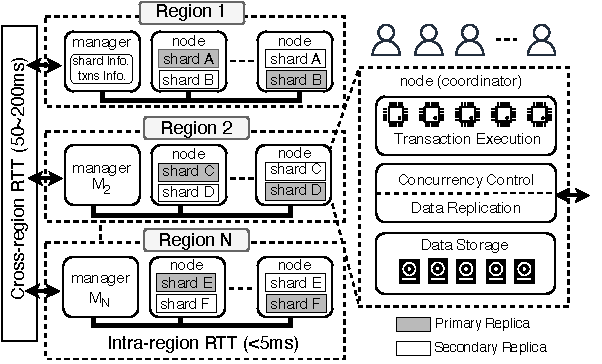
\includegraphics[width=\columnwidth]{figures/deployment.pdf}
\vspace{-10pt}
  \caption{This diagram presents a typical deployment for multi-region databases. The database is partitioned into multiple data shards spanning over multiple regions. Each shard includes a primary replica and several secondary replicas. Intra-region communications are much faster than inter-region communications.}\label{fig:intro}
  \vspace{-10pt}
\end{figure}

In reality, existing consistency models tend to be either overly strong or can be further enhanced without performance degradation. Aggressive models (e.g., strict serializability model ~\cite{papadimitriou1979serializability}) abstract the entire system as a single node, necessitating heavy synchronizations between all computing servers. This approach leads to poor performance in multi-region deployments. Moreover, this model fails to preserve the advantages of near-client computing: even a local transaction has to be ordered with cross-region ones, which is at odds with the motivation of multi-region deployment. Other models provide weaker consistency (e.g., strong snapshot isolation~\cite{daudjee2006lazy}). While these models may suffice for certain application scenarios, the consistency guarantees for local transactions can be further enhanced without much performance overhead: the communication cost for coordinating local transactions can be cheap when using modern hardware and networks. 

% These models use uniform standards for all types of transactions


% (P.3 Many new serializable databases have been proposed, but
% they lack a unified consistency level.)

In this paper, we propose region-linearizable serializability (for short, RLS), the first consistency model to provide as strong as possible consistency for multi-region databases. RLS treats CRTs and IRTs differently. It ensures strict serializability (i.e., the strongest consistency guarantee) for IRTs from the same region and provides regular serializability for CRTs. Specifically, RLS ensures serializability and ``no stale reads'' property (a.k.a. regularity) for all transactions (i.e., both CRTs and IRTs) while preserving real-time order only for the transactions that at least access one same region. For a formal definition, we refer readers to \chref{sec:model}.



To demonstrate the efficiency and applicability of RLS, instead of creating a new transaction protocol from scratch, we design, implement, and evaluate variations of two database systems: Spanner and CockroachDB (for short, CRDB). We refer to these variants as Spanner-RLS and CRDB-RLS, respectively. We chose these two database systems because they complement each other in both the consistency model (strict serializability versus single-key linearizability) and the design of concurrency control protocols (two-phase locking versus timestamp ordering). These two proof-of-concept prototypes pave the way for efficient and practical optimization of distributed protocols when deployed across multiple regions based on a correct-by-construction approach.

Specifically, Spanner and Spanner-RLS follow the design of traditional pessimistic concurrency control: it orders transactions using locks and commits transactions using the two-phase commit. Our variation (Spanner-RLS) significantly reduces CRTs' contention footprint (i.e., locking duration), thus allowing more parallel concurrency. As a result, Spanner-RLS attains $1.16\times$ to $89.01\times$ higher throughput than Spanner while having similar latency.

We present CRDB-RLS as a practical example to demonstrate that databases using weaker consistency models can also benefit from RLS by tightening their consistency guarantees. 
The original consistency model (i.e., single-key serializability) used by CRDB is considerably weaker than RLS.
We implemented regional semantics into CRDB's conflict detection protocol, requiring all conflicting IRTs to be ordered within the regions, even if they access different keys. Given that intra-region communication is significantly cheaper than cross-region communications, the performance overhead of CRDB-RLS can be ignored (e.g., less than $\sim15\%$ in our evaluation). Conversely, the stronger guarantee efficiently eliminates anomalies caused by violating the real-time order, thus simplifying application development~\cite{spanner:osdi12, lu2023ncc}.

\vspace{3pt}
\noindent\textbf{Contributions.} In summary, this paper's contributions stem from a fundamental insight that existing consistency models are inadequately designed for multi-region deployment. To our knowledge, this paper provides the first tailored consistency model for multi-region transactional processing. Our contributions are four-fold: 

\vspace{3pt}
\begin{itemize}[leftmargin=*, itemsep=3pt]
\setlength{\parsep}{0pt}
\setlength{\parskip}{0pt}
\setlength{\parindent}{1em}
  \item We systematically analyze the multi-region deployment model and highlight the limitations of existing consistency models.
  \item We implemented two distinct system variations, Spanner-RLS and CRDB-RLS, to demonstrate the efficiency and applicability of our novel consistency model (RLS). Both of the two prototypes are built on open-source codebases, and the source code is available at {\color{darkred}{\url{https://github.com/vldb24p771/spanner_rls}}} and {\color{darkred}{\url{https://github.com/vldb24p771/crdb_rls}}}, respectively.
  \item We extensively evaluate these variations and present compelling results showcasing the substantial performance improvements achieved by RLS. Specifically, RLS enhances Spanner's performance, achieving throughput improvements ranging from $1.16\times$ to $89.01\times$, and provides more robust consistency guarantees for CRDB without significant performance degradation.
  \item Spanner-RLS and CRDB-RLS can serve as practical templates for the future adoption of RLS to other concurrency control protocols.
% \vspace{1pt}
\end{itemize}
\vspace{6pt}


The rest of the paper is organized as follows. \chref{sec:background} discusses the system model of our multi-region databases deployment, the background of geo-distributed transaction processing, and the motivating applications. \chref{sec:model} details our new consistency model: RLS. \chref{sec:spanner} illustrates the application of RLS to Spanner.  \chref{sec:crdb} delves into CRDB and CRDB-RLS. Finally, a discussion of related works is presented in  \chref{sec:related}, and  \chref{sec:conclusion} concludes the paper.


\section{Background and Motivation}\label{sec:background}
This section provides background on multi-region databases and the issues of existing geo-distributed transaction protocols. 


\begin{table*}[]
  \renewcommand\arraystretch{1.15}
    \begin{tabular}{cccc} \hline
    System      & Transaction Protocol                                        & Consistency  Models       & Coordination Blocking \\ \hline
    Spanner~\cite{spanner:osdi12}     & Read-write: 2PL + 2PC;  Read-only:   TSO                    & SS        & Yes                         \\
    Calvin~\cite{calvin:sigmod12}      & Centralized coordinator                                     & SS        & Yes                         \\
    Slog~\cite{slog:vldb19}        & CRT: Centralized coordinator;  IRT:   Intra-region Sequencer & SS        & Yes                         \\
    Detock~\cite{nguyen2023detock}      & CRT: Dependency-graph;  IRT:   Intra-region Sequencer        & SS        & Yes                         \\
    Janus~\cite{janus:osdi16}       & Dependency-graph                                            & SS        & Yes                         \\
    Epaxos~\cite{epaxos:sosp13}      & Dependency-graph                                            & SS        & Yes                        \\
    Ocean Vista~\cite{ov:vldb19} & TSO  (Watermark)                                            & SS        & Yes                         \\
    CRDB~\cite{taft2020cockroachdb}        & TSO (HLC)                                                   & SKL & Yes                         \\
    RedT~\cite{zhang2023redt}        & 2PL + 2PC                                                   & Serial.              & Yes                         \\
    Tapir~\cite{tapir:tocs}       & Variant of OCC                                              & Serial.              & No (by aborting IRTs)      \\
    MDCC~\cite{mdcc:eurosys13}        & Paxos                                                       & SI      & Yes            \\  \hline          
    \end{tabular}
    \caption{This table summarizes the state-of-the-art geo-distributed transaction systems in the literature. These existing systems either block  IRTs or enforce the IRTs to abort when the IRTs conflict with an ongoing CRT.}\label{tab:compare}
    \vspace{-5pt}
\end{table*}

\begin{figure}[t]  
    \centering
    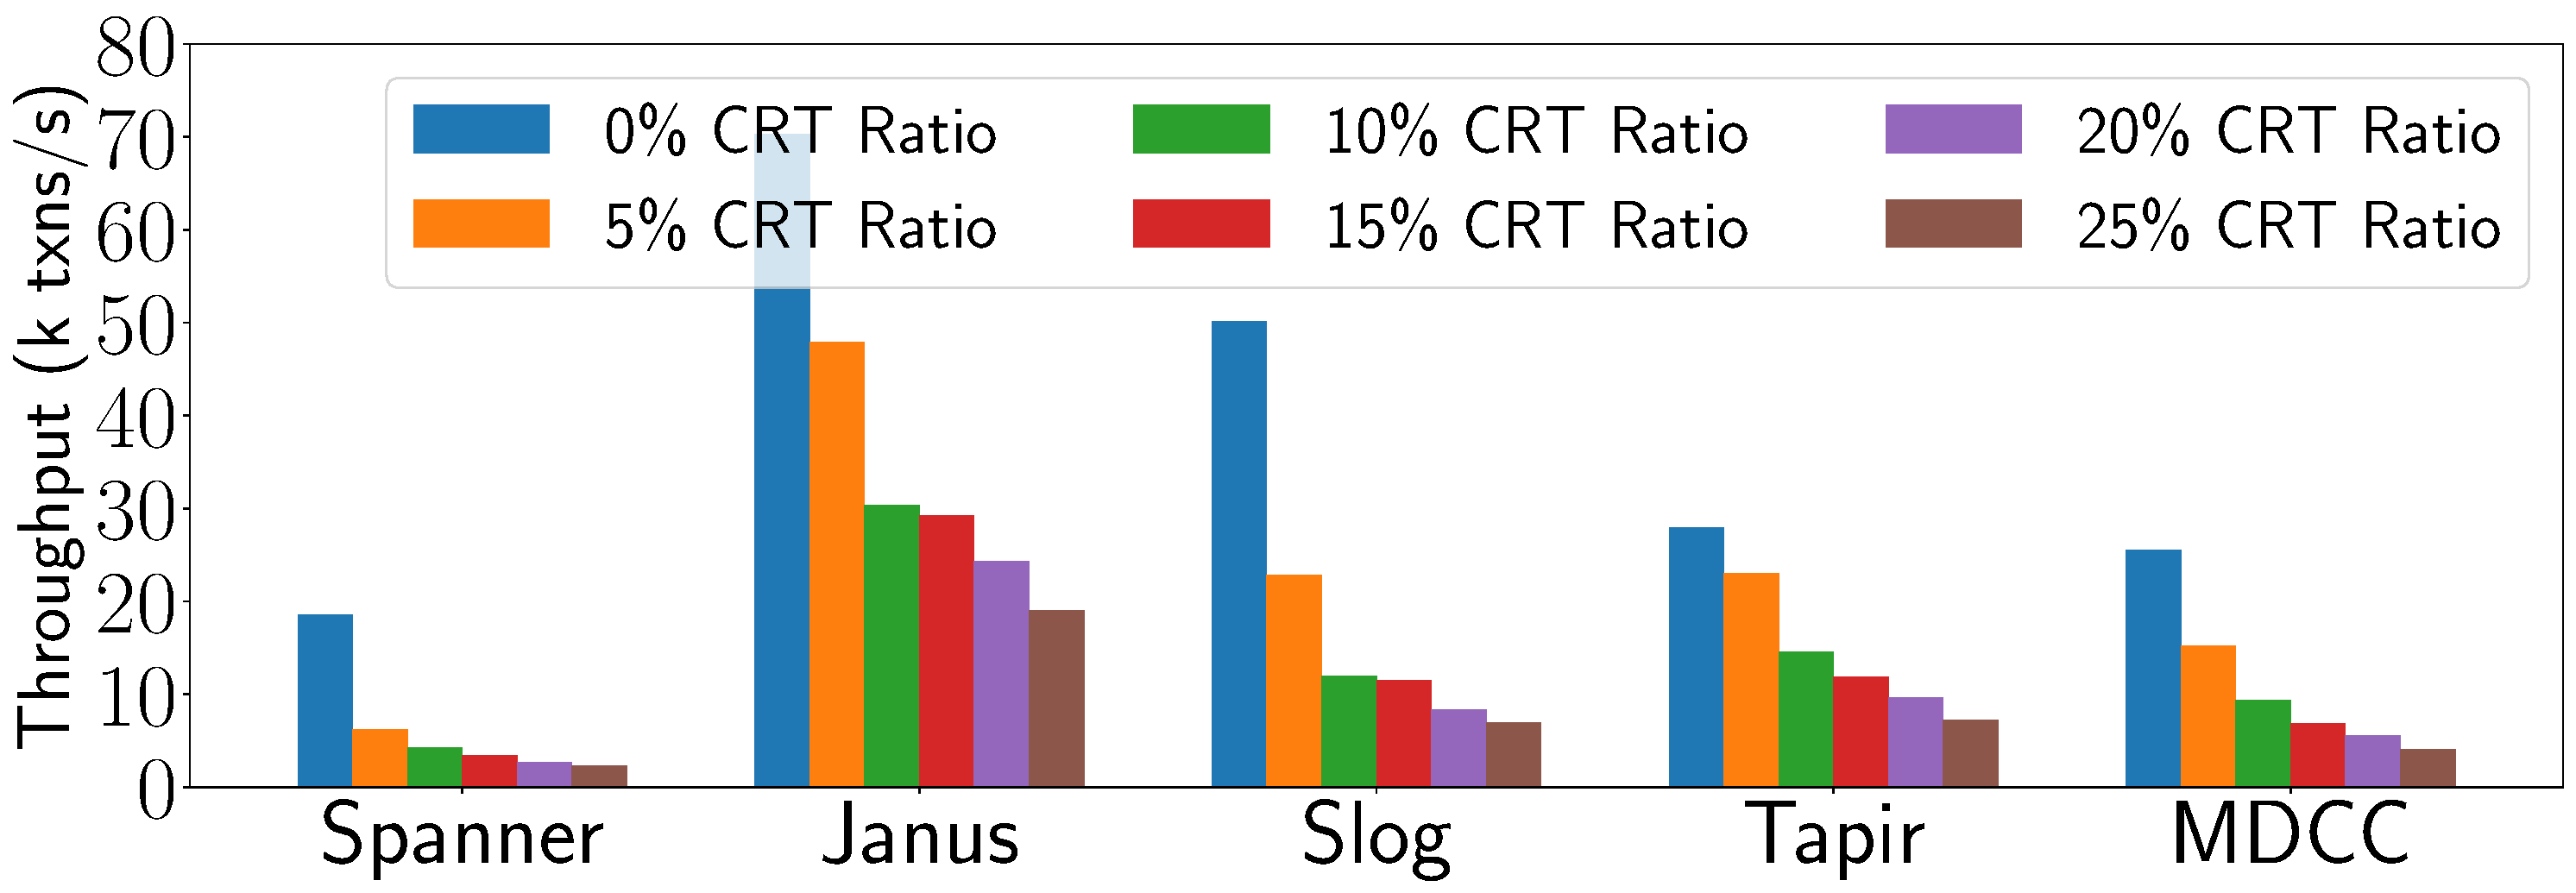
\includegraphics[width=1\columnwidth]{eval-figs/CRT_perf.pdf}
  \vspace{-15pt}
    \caption{Impact of CRT ratio on the throughput of the state-of-the-art geo-distributed transaction systems.}\label{fig:crt}
    \vspace{-5pt}
\end{figure}

\subsection{Multi-region Databases}\label{sec:background:deployment}
Multi-region infrastructures motivate our design of RLS. Deploying a multi-region application has the following advantages. 


\begin{itemize}[leftmargin=*, itemsep=1.5pt]
  \setlength{\itemsep}{0pt}
  \setlength{\parsep}{0pt} 
  \setlength{\parskip}{0pt}
  \setlength{\parindent}{1em}
    \item \textbf{[Low data access latency]} Multi-region deployment enables the placement of data in proximity to active client concentrations across different regions. Applications are designed to predominantly access a data shard from a single region, resorting to cross-region data access only when necessary. This approach facilitates applications in offering global data access with ultra-low latency.
    \item \textbf{[Meet data governance policy]} Privacy regulations impose multi-region deployments for global services with strict requirements on data residency. For instance, the General Data Protection Regulation (GDPR) forbids replicating European citizens' data outside. Thus, multi-region deployments are becoming the de facto choice for multinational companies.
    \item \textbf{[Flexible failure model]} Multi-region deployment allows for data replication across regions, significantly enhancing availability by tolerating complete region failures. In practice, replicating data globally can be costly. Users have the flexibility to define distinct replication policies based on data criticality, such as replicating critical data across regions and keeping other data within the same region.

    

\end{itemize} 



A typical multi-region deployment model is illustrated in \fig{fig:intro}. The database is partitioned into multiple data shards spanning over multiple regions. Each shard comprises a primary replica and several secondary replicas. Replicas can be configured to reside in cross-region or intra-region nodes (servers) based on replication policies. Each region is equipped with a centralized transaction manager responsible for globally consistent metadata (e.g., table schema, data placement policy, and globally unique transaction IDs). Nodes can communicate with each other over the network. Our assumptions include a partially synchronized network, and every message in the database is eventually delivered and processed.
% This new consistency model is especially suitable for emerging mission-critical edge computing applications as this model not only provides strong isolation (i.e., serializability) and real-time order within each region but also has the unique potential of providing stable low latency and availability for single-region transactions (SRT).

\subsection{Geo-distributed Transaction Protocols}\label{sec:background:geo}

Many influential works have been proposed to optimize the performance of geo-distributed transaction processing. We summarize the state-of-the-art systems in \tab{tab:compare}. All of these systems support at least serializability as their consistency model or can be enhanced to serializability with minor modifications (e.g., MDCC).

Generally, these systems focus on optimizing the cost of coordinating transactions from the protocol scope. For instance, some works attempt to reduce either the number or the overhead of network round-trips in transaction coordination. Tapir~\cite{tapir:tocs} improves Spanner's performance by integrating two-phase commit and consensus protocols into a single framework, eliminating redundant coordination and reducing the WAN round-trips. RedT~\cite{zhang2023redt} enhances system performance by further decreasing the network round-trips. RedT targets RDMA-capable networks for local communication and employs a pre-write-log mechanism to eliminate the synchronization of \texttt{prepare} messages (i.e., the first phase in two-phase commits) from the coordinator to primary replicas.


Calvin~\cite{calvin:sigmod12}, Slog~\cite{slog:vldb19}, Detock~\cite{nguyen2023detock}, Ocean Vista~\cite{ov:vldb19}, Epaxos~\cite{epaxos:sosp13}, MDCC~\cite{mdcc:eurosys13}, and Janus~\cite{janus:osdi16} follow the design of deterministic databases, which logically create a global log containing all transactions that have been input into the system. The system then ensures a concurrent execution schedule equivalent to processing all transactions serially in the order they appear in this log (i.e., a partial order). Consequently, after the transaction order is determined, the execution of both CRTs and IRTs can be local. The executors adhere to orders in the logs they receive.

However, all these proposals can not essentially prevent an IRT from being blocked by CRTs (as illustrated in \chref{sec:rls:issue}). Briefly, Spanner and RedT employ two-phase locking for transaction ordering and commit transactions using two-phase commit. When an IRT conflicts with an ongoing CRT, the IRT has to be blocked for the required locks. Tapir uses a variation of OCC and enforces the IRT to abort in the validation phase, resulting in a high abort rate (as confirmed by other previous papers~\cite{ov:vldb19, chen2021achieving}). Determinisct databases either order IRTs and CRTs together (e.g., Calvin, Janus, Epaxos, and Ocean Vista) or require an IRT to be blocked, waiting for the execution of CRTs that are scheduled ahead (e.g., Slog and Detock) for overly strong consistency guarantees.


Consequently, these systems can cause severe performance issues when CRTs occur in the database, and the contention between the IRTs and CRTs is relatively high. We experimentally studied the impact of CRT ratios on the five latest representative systems in \fig{fig:crt}. We used YCSB-T workloads with a Zipf parameter of 0.8. For detailed evaluation setups, we refer readers to \chref{sec:spanner:eval}. From the experimental results, our key observation is that even a few CRTs can significantly degrade the whole system's performance (e.g., up to $86\%$ degradation with only $5\%$ CRTs).



RLS addresses such issues by rethinking the limitations within existing consistency models and thus is fundamentally different from these proposals. RLS trades off consistency for performance with minimal intrusion (i.e., the consistency tradeoff in RLS is tightly necessary for addressing blocking issues). We regard RLS as orthogonal to these advanced geo-distributed transaction protocols. Consequently, new protocols may benefit from the methodology of RLS and the key optimizations of these advanced protocols.

\section{Region-linearizable Serializability}\label{sec:model}

In this section, we formally define our new consistency model: Region-linearizable Serializability (RLS), which is specially tailored for the database systems that are deployed in near-client computing facilities (e.g., Regions~\cite{aws:region} in AWS). For comparisons with other serializable consistency models, we refer readers to \chref{sec:rls:compare}.

\subsection{Definition of RLS}\label{sec:model:def}

For clarity, we adopted the formalism from existing works~\cite{rss}. \tab{tab:model} summarizes the notations used in our definition, which will be further illustrated later.
Without loss of generality, we consider an OLTP service (either a relational database or a transactional key-value store) handling data objects identified by unique keys. We use $\mathcal{K}$ to represent the global key spaces. $\mathcal{K}$ is divided into multiple disjoint \textit{shards} to facilitate transaction processing across many nodes (servers), which is common in multi-region deployed data-intensive applications.

\vspace{2pt}
\noindent\textbf{Shard Groups (e.g., grouped by regions)}. Grouping 
semantics is one of the foremost distinctions of \xxcons compared to other serializable consistency models. Specifically, \xxcons divides data shards into disjoint groups and 
ensures linearizability (i.e., the strongest consistency) for intra-group operations. For inter-group operations, RLS provides regular serializability.

Note that grouping and sharding construct a two-level division of 
the global key space ($\mathcal{K}$): the OLTP service has many disjoint groups,
and each group contains a number of (not necessarily equivalent) disjoint 
shards. This division serves different purposes; sharding is for horizontally scaling the 
service to run on many servers, and the division policy 
is usually for reducing the ratio of cross-shard transactions to achieve 
high efficiency~\cite{nguyen2023detock}.
On the other hand, grouping is a consistency strategy where cross-group external ordering requirements are typically less important. Such semantics are usually related and directed by geo-distributed (multi-region) deployments. 

We regard this two-level framework as essential because it efficiently bridges the division based on application semantics (e.g., the data items grouped by warehouse ID in TPC-C~\cite{tpcc}) and division based on deployment topology (e.g., the data shards grouped by regions in geo-distributed deployments).

\vspace{2pt}
\noindent\textbf{Transactions and Operations}. Clients interact with the OLTP service through transactions. Each transaction comprises several single-key read or single-key write \textit{operations}. Formally, each transaction $T$ is a tuple $(\Sigma_T, \xrightarrow{to})$, where $\Sigma_T$ is the set of operations in $T$, and $\xrightarrow{to}$ is a total order on $\Sigma_T$. Each operation is either a read (denoted as $o_1 = r(k_1, v_1)$) or a write (denoted as $o_2 = w(k_2, v_2)$). We use $\mathcal{R}_T = \{k | r(k, v) \in \Sigma_T\}$ to denote $T$'s read set and $\mathcal{W}_T = \{k | w(k, v)\} \in \Sigma_T\}$ as $T$'s write set. 

It should be noted that RLS, as a consistency model, does not essentially require the read and write set of each transaction to be determined upfront, which is a common but restrictive assumption in existing deterministic databases~\cite{slog:vldb19,calvin:sigmod12,mdcc:eurosys13,epaxos:sosp13, nguyen2023detock}. Essentially, RLS supports general transaction semantics (to be illustrated in our example system: Spanner-RLS, \chref{sec:spanner}). In RLS, we consider a general transaction $T_1 = \{r(x, n), w(n, v)\}$ that reads the value of key $x$ as the key for the write operation, where  $\mathcal{W}_{T1}$ can not be obtained before execution.

\begin{table}[]
    \vspace{5pt}
    \small
    \renewcommand\arraystretch{1.35}
    \setlength{\tabcolsep}{1.25pt}
    \begin{tabular}{|c|c|l|}
    \hline
    \multirow{3}{*}{Ops}    
    & $o$  & Database operation, e.g., read, write, insert, scan.               \\ \cline{2-3}
    & $r(k, v)$  & Read the value $v$ using key $k$               \\ \cline{2-3}                   
          & $w(k, v)$ & Write value $v$ for key $k$       \\ \hline

    \multirow{4}{*}{Txns}    
    & ${T}$  & Txn consists of operations ($\Sigma_T$) with order ($\xrightarrow{to}$)               \\ \cline{2-3}
    & $\mathcal{R}_{T}$  & Read Set of Transaction T                \\ \cline{2-3}                   
          & $\mathcal{W}_{T}$ & Write Set of Transaction T          \\ \cline{2-3}
          & $\mathcal{G}_T$  & The set of all shard groups relevant to $T$                      \\ \hline
    \multirow{2}{*}{Data}  & $\mathcal{K}$    &  Global Key Space                      \\ \cline{2-3} 
                             & $g$   & A shard group contains multiple shards                      \\ \hline
    \multirow{6}{*}{\makecell{Order}}
                
                                        & $\mathcal{H}_i$   & Transaction history on $node_i$, $\mathcal{H}_i =$ $(\mathcal{E}_i, {po}_{i}, {\tau}_i)$                            \\ \cline{2-3} 
                              & $\mathcal{H}$   & Transaction history of the whole system, $\mathcal{H} =$ $\bigcup \mathcal{H}_i$                            \\ \cline{2-3} 
                              & $\mathcal{S}$   & Totally ordered serializable schedule for all txns                           \\  \cline{2-3} 
                              & $\xrightarrow{rb}$   & Real-time order imposed by runtime execution                           \\  \cline{2-3} 
  
                              &  $\xrightarrow{so}$    & Oreder for operations in   $\mathcal{S}$                                      \\ \cline{2-3} 
                              &   $<_S$   &  Oreder for transactions in   $\mathcal{S}$               \\ \hline
    \end{tabular}
    \vspace{2pt}
    \caption{Preliminaries and notations for RLS.}\label{tab:model}
    \vspace{-5pt}
    \end{table}

\vspace{2pt}
\noindent\textbf{Conflicts and Relevance.}
We say two transactions conflict with each other if they access the same key, and at least one of the two accesses is ``write'' (which is known as read-write conflicts and write-write conflicts in other papers). We say a transaction $T$ is relevant to shard group $g$ if $T$ accesses at least one key owned by $g$, and we use $\mathcal{G}_T$ to represent the set of all groups relevant to $T$. Formally, $$\mathcal{G}_T = \{g\ |\ \exists k: k \in g \land k \in (\mathcal{W}_T \cup \mathcal{R}_T)\}$$

\vspace{2pt}
\noindent\textbf{History and Equivalence.} A history of a data $node_i$ ($server_i$) is an associative triple $\mathcal{H}_i =$ $(\mathcal{E}_i, {po}_{i}, {\tau}_i)$, where $\mathcal{E}$ is a set of operations; $po$ is a partial ordering on $\mathcal{E}$ into processes; and $\tau$ divides $\mathcal{E}$ into transactions. We say two histories ($\mathcal{H}_1$ and $\mathcal{H}_2$) are equivalent if they have the same $\mathcal{E}$, $po$, and $\tau$. Intuitively, two equivalent histories have the same sequence of operations for each client process and thus are indistinguishable inside the database. 

\vspace{2pt}
\noindent\textbf{Real-time order.} An order of transactions is usually considered as a set of \textit{return before} relations~\cite{lamport2019time}. In our paper, we say a transaction $T_1$ precedes another transaction $T_2$ if $T_1$ finishes (commits) before $T_2$ starts (i.e., arrives at the database system), denoted as $T_1 \xrightarrow{rb} T_2$.

\vspace{5pt}

\noindent\textbf{\textit{Definition of \xxcons}}. We then define RLS using the notations above. We say that an OLTP service ensures \xxcons, if for all execution histories, $\mathcal{H} =$ $\bigcup \mathcal{H}_i$, are equivalent to a serial schedule $\mathcal{S}$ and the following three properties hold for $\mathcal{S}$.


\begin{itemize}[leftmargin=*, itemsep=1.5pt]
    \setlength{\itemsep}{0pt}
    \setlength{\parsep}{0pt}
    \setlength{\parskip}{0pt}
\item \textit{\underline{Serializability.}} There exists serial schedule $\mathcal{S}$ with total ordering $so$ on $\mathcal{E}$ such that \circled{1}
$S$ is equivalent to $H$; and \circled{2} no two transactions overlap in $so$, i.e., either 
    \vspace{2pt}
$$o_1 \xrightarrow{so} o_2,  \forall o_1 \in T_1, \forall o_2 \in T_2$$ or 
$$o_2 \xrightarrow{so} o_1,  \forall o_1 \in T_1, \forall o_2 \in T_2$$
    \vspace{2pt}
Therefore, the property \circled{2} infers that $\xrightarrow{so}$ defines a total order $<_S$ among all transactions.

    \vspace{2pt}
\item \textit{\underline{No Stale Reads.}} Formally, for any two transactions $T_1$ and $T_2$

$$ \mathcal{W}_T \cap (\mathcal{W}_T \cup \mathcal{R}_T) \neq \emptyset \land T_1 \xrightarrow{rb} T_2 \implies T_1 <_S T_2$$

    \vspace{2pt}
\item \textit{\underline{Real-time Ordering inside all Shard Groups.}} Formally,
$$\mathcal{G}_{T_1} \cap \mathcal{G}_{T_2} \neq \emptyset \land T_1 \xrightarrow{rb} T_2 \implies T_1 <_S T_2$$
\end{itemize}




\subsection{Performance Issues in Strict Serilizability}\label{sec:rls:issue}

Strict serializability (SS), the most substantial consistency level for distributed databases, ensures that a replicated distributed database works as a single node that executes all client transactions serially. The serial order respects the real-time relations (i.e., the ``return before'' relation in \chref{sec:model:def}) among all client transactions. 

However, the strong guarantees of SS always come up with high-performance costs, especially when deployed in a multi-region environment. This has led both academia and industry to seek weaker consistency models. For example, numerous new consistency models were proposed in recent years (see \chref{sec:rls:compare}), and almost all industrial systems do not provide SS by default.

\subsection{Practical Implications}\label{sec:rls:practical}

In essence, the guarantee of SS is considered excessive for many multi-region application scenarios. Specifically, ensuring a real-time relation between transactions pertains to external (out-of-band) causal relations among transactions. 
Since a system is unaware of external relations, SS regards \textit{all} pairs of transactions without overlapping lifetime as potentially causally related and pertains to their ordering, albeit most transactions are independent. 
 
\xxcons ensures the ``no stale reads'' property for all transactions, effectively preventing most application-level anomalies~\cite{viotti2016consistency}. Additionally, \xxcons enforces real-time ordering among transactions accessing interleaved regions (i.e., conflict IRTs and CRTs), including transaction ordering requirements inferred by transitivity. Compared to SS, the only anomalies in \xxcons may arise from the potential disruption of real-time ordering among transactions happening independently within non-overlapping regions. 

We argue that such anomalies do not compromise the correctness of multi-region databases for two primary reasons. First, multi-region databases optimally leverage data access locality to assign shards to regions (see \chref{sec:background:deployment}). Typically, each region manages (e.g., being the leader of) shards containing data of nearby clients, making two transactions accessing non-overlapped regions causally unrelated. Thus, prioritizing their real-time order will not introduce application-level anomalies. 


Second, the time window for breaking causal relations is narrow. \xxcons necessitates ``no stale reads'' for all transactions, whether intra-region or cross-region. To sever the causal relationship between two transactions, external communication must conclude faster than a transaction's lifetime. 
Specifically, consider two transactions $T_2$, $T_3$ accessing non-overlapped regions, where $T_2 \xrightarrow{rb} T_3$. If anomalies were present, it would imply the existence of another transaction $T_1$ accessing both $T_2$ and $T_3$'s regions, leading to a final serial order of $T_3 <_S T_1 <_S T_2$ (as depicted in \fig{fig:rls_ss}). However, as \xxcons also mandates ``no stale reads'', $T_1$ must be concurrent with $T_2$ and $T_3$, implying that the external causal relation must conclude within $T_1$'s lifetime. 


Therefore, \xxcons possesses the unique potential to significantly enhance the scalability and latency of multi-region databases while maintaining correctness and programmability. \xxcons stands out as the pioneering consistency model that takes into account real-world deployments and the inherent locality feature of data.


\begin{figure}[t]  
    \centering
    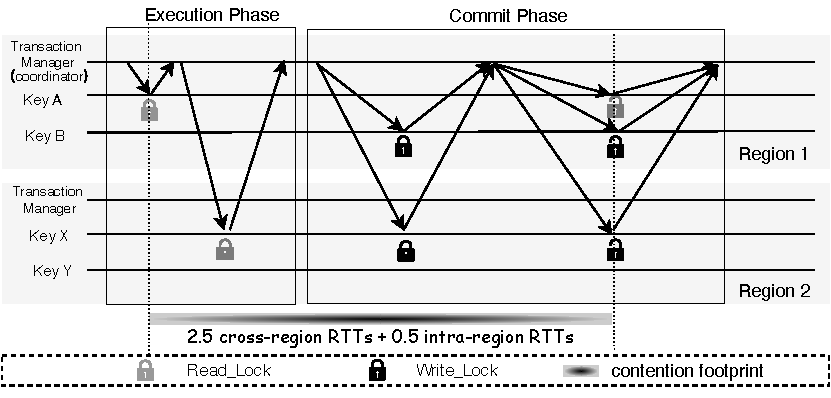
\includegraphics[width=1\columnwidth]{figures/spanner.pdf}
	\vspace{-5pt}
    \caption{This diagram shows how Spanner orders a CRT using 2PL and commits it using 2PC in a multi-region deployment. Replicas are removed for readability.} \label{fig:spanner}
	% \vspace{-5pt}
\end{figure}

\section{\spanner and \spannerxx}\label{sec:spanner}
In this section, we present the design, implementation, and evaluation of Spanner and Spanner-RLS. We regard Spanner-RLS as a specific instance of using our new consistency model (RLS) to advance the performance of existing strictly serializable databases. 

\subsection{Protocols and Implementations}

\noindent\textbf{\spanner Background.} Google's \spanner provides strict serializability (a.k.a. external consistency) for read-write transactions by coordinating them using two-phase locking (2PL) and then committing the transactions using two-phase commit (2PC). 

\fig{fig:spanner} presents an example, where a transaction $T$ reads the keys $A$ and $X$, and then updates the keys $B$ and $X$. The keys $A$ and $B$ are located at different data nodes in $region$ $1$, and the key $X$ is located at a data node in $region$ $2$. To commence, $T$ is forwarded to the transaction manager that $T$ firstly accesses, acting as the coordinator and assigning a globally unique \texttt{TID} to $T$. In this example, the transaction manager of $region$ $1$ serves as the coordinator since $T$ reads the key $A$ in the first access. Subsequently, the coordinator sequentially executes all the transaction operations. During execution, it acquires read locks for each read operation and buffers write operations in temporary memory. After buffering all writes, the coordinator obtains exclusive locks for all write keys (i.e., the keys $B$ and $X$) and installs the writes if all the required locks are acquired. Following this, all the locks (both read and exclusive locks) are released immediately. As such, $T$ is successfully executed and committed.

We are now prepared to introduce the performance issues in Spanner. Spanner coordinates intra-region transactions (IRTs) and cross-region transactions (CRTs) similarly, where a read lock held by a CRT will block all writes from both CRTs and IRTs, and an exclusive lock held by a CRT will prevent all reads and writes, correspondingly. Consequently, a CRT's contention footprint (i.e., the lock duration) is extremely large. More than two cross-region network round trips will block all conflict transactions. In our example, it takes $2.5$ cross-region network round trips and $0.5$ intra-region round trips. Even worse, such blockings can rapidly accumulate through transitive relations. For instance, considering another CRT $T^{\prime}$ that accesses the key $B$ and $Y$, $T^{\prime}$ can successfully acquire the exclusive lock on the key $Y$ while having to wait for the lock on the key $B$. Consequently, all other IRTs and CRTs that access the key $Y$ have to compete with $T^{\prime}$ for ownership of the lock on the key $Y$, enlarging the affected key space.



\begin{figure}[t]  
    \centering
    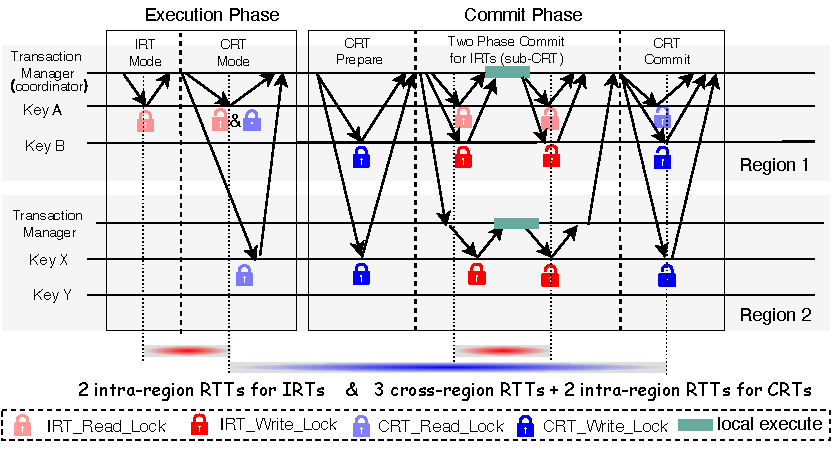
\includegraphics[width=1\columnwidth]{figures/RLS-spanner.pdf}
    \caption{This diagram shows how Spanner-RLS orders a CRT using a variant of 2PL and commits it using 2PC.} \label{fig:spannerrls}
\end{figure}

\SetKwProg{Fn}{function}{:}{}

\SetKwFunction{Coordsp}{Coord-\spxx}
\SetKwFunction{FgetPreLock}{getCrossLock}
\SetKwFunction{FsetPreLock}{setCrossLock}
\SetKwFunction{FgetLock}{getInLock}
\SetKwFunction{FsetLock}{setInLock}
\SetKwFunction{FsendPrepareOK}{sendPrepareOK}
\SetKwFunction{FsendRetry}{sendRetry}
\SetKwFunction{FsendCommitted}{sendCommitted}

\SetKwData{DKey}{key}
\SetKwData{DTxn}{txn}
\SetKwData{PreLock}{crossLock}
\SetKwData{Lock}{inLock}

\SetKwData{UNLOCKED}{unLock}
\SetKwData{RLock}{readLock}
\SetKwData{WLock}{writeLock}
\SetKwData{RWLock}{readWriteLock}
\SetKwData{PreLockHolder}{crossLockHolder}
\SetKwData{LockHolder}{inLockHolder}
\SetKwProg{Event}{Event}{}{end}
\SetKwData{TouchedR}{touchedRegions}

\SetKwData{DRegion}{r}


\begin{algorithm}[t]
	\setstretch{1}
	\small 
  	\Fn{Execution phase}{
      \texttt{read\_set} \&  
      \texttt{write\_set} $\gets \emptyset$ \\
      txnType $\gets$ IRT  \Comment{Start a new transaction as IRT.}\\
       \TouchedR $\gets \emptyset$  \Comment{Regions involved in the transaction.} \\
  \LeftComment{Execute the transaction commands, which triggers the events:}\\
  \Event{$read (\texttt{key}$)}{
    
    $\texttt{value} = find\_record(\texttt{key})$ \\
    $\texttt{read\_set}.append(\texttt{key})$ \\
    \tikzmk{A}
    \TouchedR $\gets$ \TouchedR $\cup$ \texttt{key.region} \\
    \If{$	\lvert \TouchedR 	\rvert \geq 2$}{
      txnType $\gets$ CRT \\
       $Release\_IRT\_Read\_Lock(k)$ $for$ $all$ $k$ $\in$  \texttt{read\_set} \\
       $CRT\_Read\_Lock(k)$ $for$ $all$ $k$ $\in$  \texttt{read\_set} \\
    }
    \uIf{txnType == IRT}{
      $IRT\_Read\_Lock(key)$ \\
    }
    \Else(){
      $CRT\_Read\_Lock(key)$
    }
  }

  \tikzmk{B} \boxit{blue}
  \Event{write (\texttt{key}, \texttt{value}) \Comment{Writes are only buffered }}{
       $\texttt{write\_set}.append(\text{\textless}\texttt{key}, \texttt{value}\text{\textgreater})$ \\
       $Execute \ Line \ 9 \sim 13$ \\
  }

  }
  \renewcommand{\boxit}[1]{\tikz[remember picture,overlay]{\node[xshift=-1.5pt,yshift=0.5pt,fill=#1,opacity=.25,fit={(A)($(B)+(.9\linewidth,.8\baselineskip)$)}] {};}\ignorespaces} 

  \Fn{Commit phase}{
      \uIf{txnType == IRT} {
        $IRT\_Write\_Lock(k)$ $for$ $all$ $k$ $\in$ \texttt{write\_set}  \\
        wait for all \texttt{ACK}s from $storage$ \Comment{Abort if fail} \\ 
        $Commit(txn)$ \\
        $Release\_IRT\_Read\_Lock(k)$ $for$ $all$ $k$ $\in$  \texttt{read\_set} \\
        $Release\_IRT\_Write\_Lock(k)$ $for$ $all$ $k$ $\in$  \texttt{write\_set} \\
      }

      \tikzmk{A} 
      \Else(){
        $CRT\_Write\_Lock(k)$ $for$ $all$ $k$ $\in$ \texttt{write\_set}  \\
        wait for all \texttt{ACK}s from $storage$ \Comment{Abort if fail} \\ 
        Send Commit to $txn$ $managers$ $in$ $r$, $r$ $\in$  \TouchedR  \\
        \LeftComment{Each transaction manager commits the transaction as IRT} \\
        wait for all \texttt{ACK}s from the $txn$ $managers$ \Comment{Abort if fail} \\ 
        $Commit(txn)$ \\
        $Release\_CRT\_Read\_Lock(k)$ $for$ $all$ $k$ $\in$  \texttt{read\_set} \\
        $Release\_CRT\_Write\_Lock(k)$ $for$ $all$ $k$ $\in$  \texttt{write\_set} \\
      } \tikzmk{B} \boxit{blue}}
	% \Fn{\Coordsp-\texttt{InRegion-Txn}}{
  %       \For{$\forall \DKey \in \DTxn.readSet$}{
  %         \PreLock $\gets$ \FgetPreLock(\DKey) \\
  %         \Switch{\PreLock}{
  %           \Case{\UNLOCKED}{}
  %           \Case{\RLock}{
  %             \PreLockHolder{\DKey} $\gets$ \PreLockHolder{\DKey} $\cup$ \{\DTxn\} \\
  %             \FsetPreLock{\DKey, \RLock} \\
  %             \textbf{break} \\
  %           }
  %           \Case{\WLock}{}
  %           \Case{\RWLock}{
  %             \If{$\DTxn \notin \PreLockHolder{\DKey}$}{
  %               \FsendRetry(\DTxn) \\
  %             } 
  %             \Else(){
  %               \FsetPreLock{\DKey, \RWLock} \\
  %             }
  %             \textbf{break} \\
  %           }
  %         }
  %       }
  %       \For{$\forall \DKey \in \DTxn.writeSet$}{
  %         \PreLock $\gets$ \FgetPreLock(\DKey) \\
  %         \Switch{\PreLock}{
  %           \Case{\UNLOCKED}{
  %             \PreLockHolder{\DKey} $\gets$ \PreLockHolder{\DKey} $\cup$ \{\DTxn\} \\
  %             \FsetPreLock{\DKey, \WLock} \\
  %             \textbf{break} \\
  %           }
  %           \Case{\RLock}{
  %             \If{$\DTxn \notin \PreLockHolder{\DKey}$}{
  %               \FsendRetry(\DTxn) \\
  %             }
  %             \Else(){
  %               \FsetPreLock{\DKey, \RWLock} \\
  %             }
  %             \textbf{break} \\
  %           }
  %           \Case{\WLock}{}
  %           \Case{\RWLock}{
  %             \If{$\DTxn \notin \PreLockHolder{\DKey}$}{
  %               \FsendRetry(\DTxn) \\
  %             }
  %             \textbf{break} \\
  %           }
  %         }
  %       }
  %       \FsendPrepareOK(\DTxn)
      % }
\caption{Algorithm of \spxx}\label{algo2}
  \end{algorithm}
% \fi

\renewcommand{\boxit}[1]{\tikz[remember picture,overlay]{\node[xshift=-30pt,yshift=0.5pt,fill=#1,opacity=.25,fit={(A)($(B)+(.9\linewidth,.8\baselineskip)$)}] {};}\ignorespaces}

\noindent\textbf{\spannerxx.} Following the methodology of our new consistency model (RLS), we treat the IRTs and CRTs differently in the variation of Spanner, termed Spanner-RLS. To achieve this, we distinguish the locks acquired by IRTs and CRTs. 
The two types of locks order transactions independently. A CRT lock does not block IRTs, and vice versa. In our design, CRT locks only provide the functionality for reservation and maintain the partial order between CRTs.


\algo{algo2} shows the pseudocode of Spanner-RLS, and we highlight the regional semantics in blue. \fig{fig:spannerrls} illustrates how Spanner-RLS executes and commits the same transaction $T$. Without loss of generality, we assume that read and write sets of a transaction are unknown to the transaction manager. Therefore, Spanner-RLS can support general transactions without prior knowledge. $T$ is firstly executed as an IRT and acquire \texttt{IRT\_Read\_Lock} for the key $A$ during the execution. $T$ switches to the CRT mode when it attempts to perform remote reads (i.e., reads the key $X$ in $region$ $2$). Before that, it releases the acquired \texttt{IRT\_Read\_Lock} for the key $A$  and updates the lock type to \texttt{CRT\_Read\_Lock}. If the key $A$ is already exclusively locked by other CRTs, $T$ aborts and directly retries using CRT mode. Otherwise, $T$ successfully enters the CRT mode and employs \texttt{CRT\_Read\_Lock} for the remaining reads (e.g., reads the key $X$).
Since all the changes are handled by intra-region communication, it will not incur much overhead. Then, following the transaction logic, $T$ computes its write set and proceeds to the commit phase. 



In the commit phase, $T$ acquire \texttt{CRT\_Write\_Lock} for the key $B$ and $X$. When all \texttt{CRT\_Write\_Lock} is successfully acquired (i.e., the order between $T$ and other CRTs has been determined), the coordinator notifies all transaction managers of the region that $T$ accessed. Each transaction manager commits $T$ independently using IRT mode. As we already allow $T$ to hold the read locks for all read keys (i.e., the keys $A$ and $X$), the read keys of $T$ can not be modified by any other CRTs. In case of any IRTs that have modified the read keys of $T$, we re-execute it locally. The tricky is that even if the re-execution depends on remote reads, we can defer the IRT lock acquisition of the execution until the remote reads have been finished since we now have obtained the read and write set of the transaction. One exception is that the transaction $T$'s read and write set may differ during re-execution, or $T$ has cycle dependency in the transaction logic (e.g., the execution in $region$ $1$ depends on the reads in $region$ $2$, the execution in $region$ $2$ depends on the reads in $region$ $1$, and both the read keys of $region$ $1$ and $region$ $2$ has been changed). In such cases, we can easily revert from Spanner-RLS to Spanner by using IRT locks directly for the CRT.

We then analyze the tradeoff in Spanner-RLS. By differentiating CRTs and IRTs locks, Spanner-RLS eliminates both the ``commit blocking'' and the ``coordination blocking'' for IRTs. In our example, the contention footprint for conflict IRTs is reduced to two intra-region network round-trip communication. On the other hand, CRTs may incur slightly more communication costs between the coordinator and the transaction managers. However, in practical workloads, IRTs are always the dominators and are more critical and sensitive to performance. In fact, if CRTs constitute the majority of the workloads, the performance degradation induced by the heterogeneous network is less of a problem. Hence, Spanner-RLS can fall back to the classic Spanner switchable at runtime.



\noindent\textbf{Read-only Transactions.} Leveraging error-bounded timing service (e.g., TrueTime API), Spanner can execute read-only transactions in a single network round trip. Using its TrueTime API, Spanner assigns a commit timestamp to each transaction, guaranteed to be between the transaction’s real start and end times. Therefore, when using the TrueTime API for read-only transactions, they can safely read from the replicas without coordination. Spanner-RLS follows this design for enhanced performance. In our evaluation, we emulated TrueTime error as 10 ms, which is used in the previous paper~\cite{rss} and matches the p99.9 value observed in practice.


\begin{figure}[t]
	\centering
	\subfloat[\footnotesize Overview\label{fig:spanner:overview:abort}]{
		  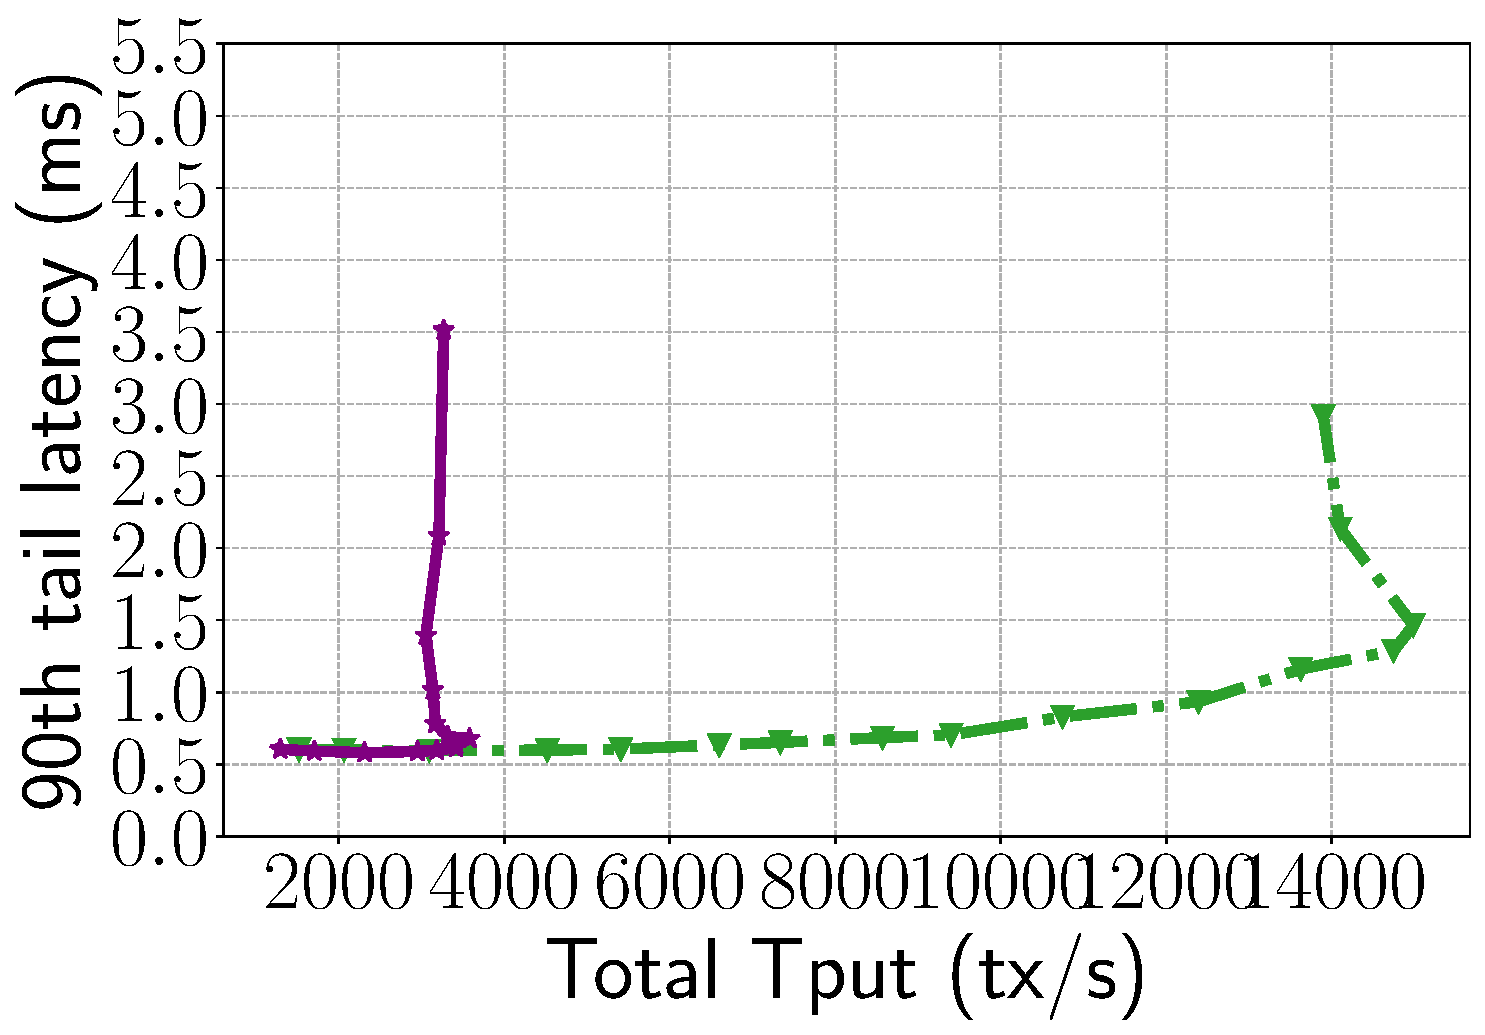
\includegraphics[width=0.45\columnwidth]{eval-figs/spanner_lat_tput.pdf}
	}
	\hfill 
	\subfloat[\footnotesize Abort Rate.\label{fig:spanner:overview:abort:breakdown}]{
		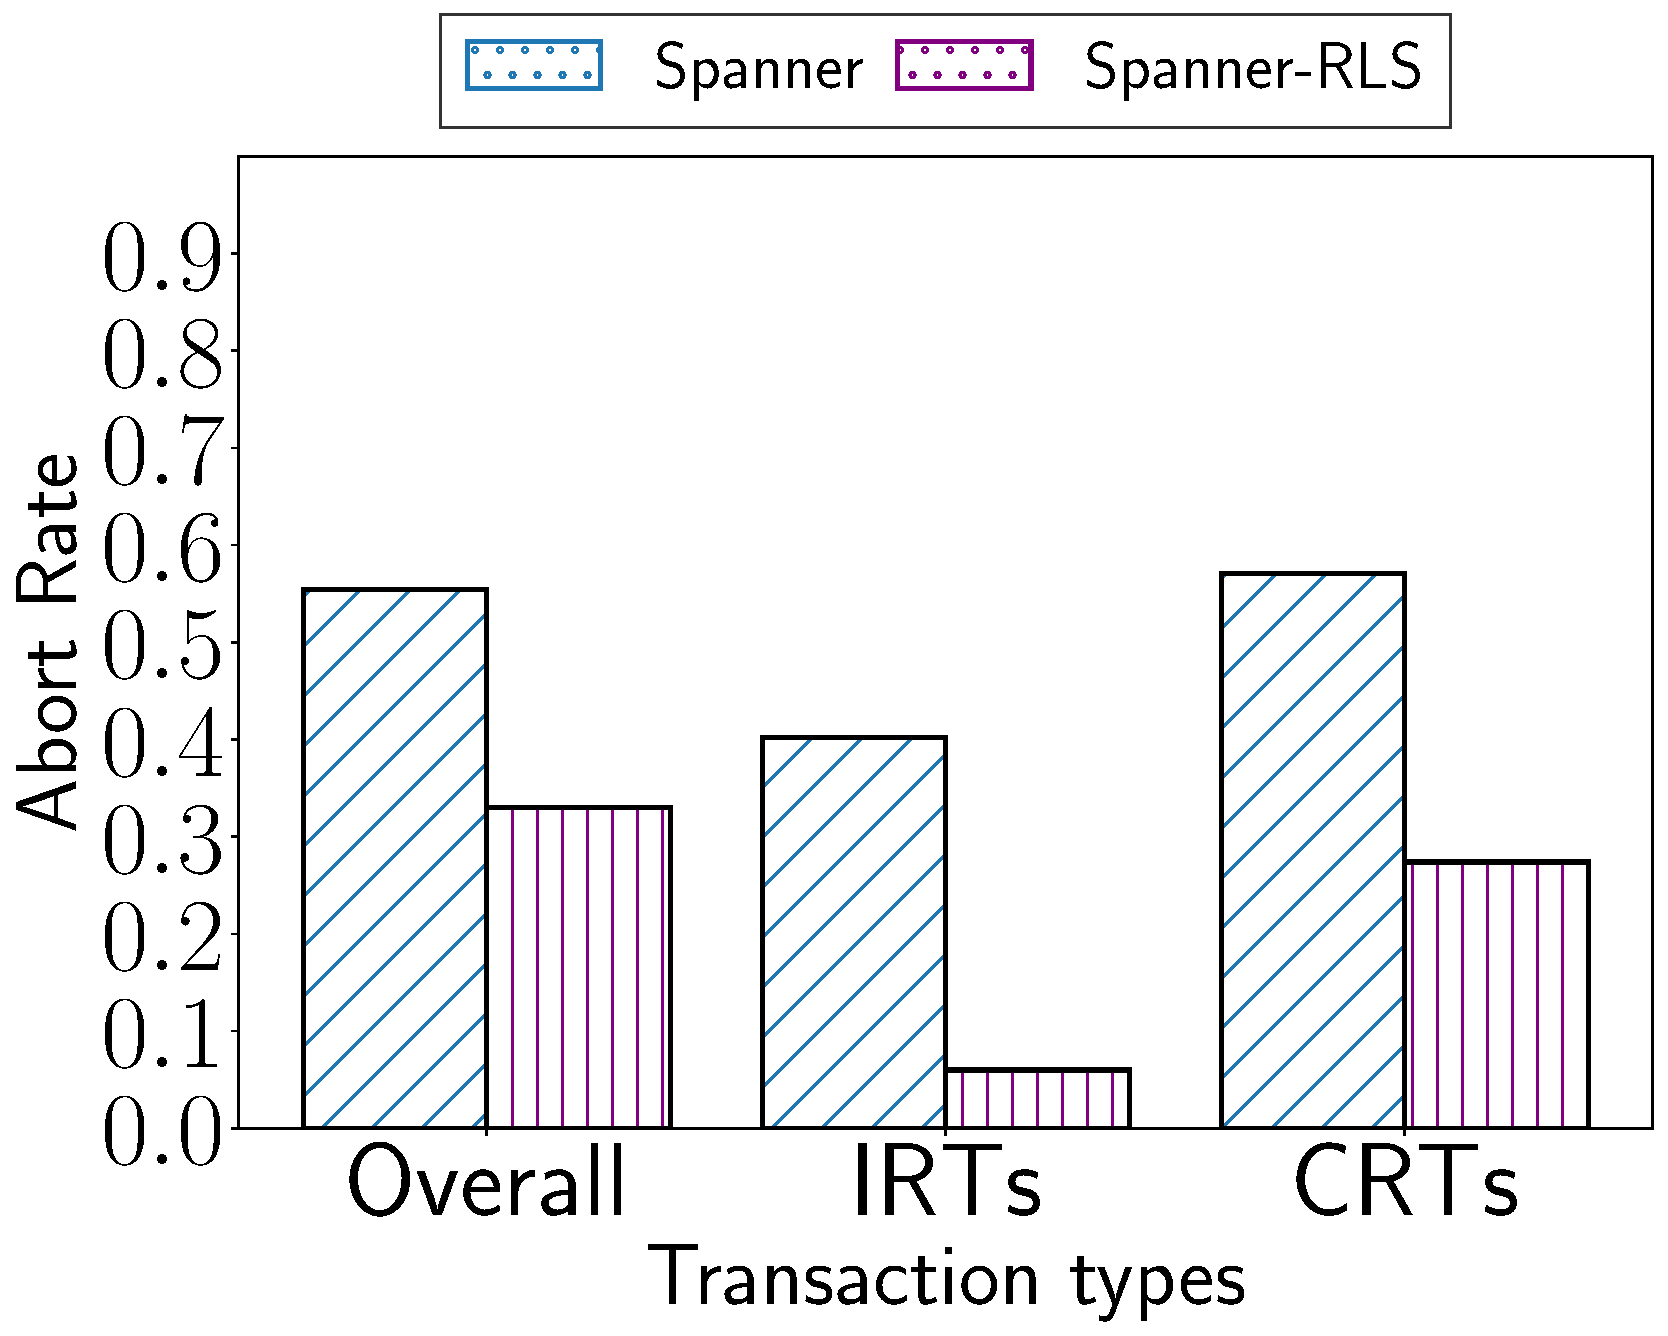
\includegraphics[width=0.45\columnwidth]{eval-figs/spanner_latency_waitdie.pdf}
	}
	\caption{Overall performance and abort rate of Spanner and Spannner-RLS on YCSB-T (default setting) using \texttt{NO\_WAIT}.}\label{fig:eval:spanner:overall:abort}
\end{figure}

\subsection{Evaluation and Discussion}\label{sec:spanner:eval}

\subsubsection{Experimental Setups} We implemented Spanner-RLS in C++ utilizing the third-party implementation~\cite{tapir:github} since the original version of Spanner is not open-sourced. We employed \texttt{libevent} for message passing between processes on distinct nodes and between threads in the same process. Transactions were implemented as stored procedures containing read and write operations over a set of keys.



\noindent\textbf{Cluster Setups.} All experiments were conducted on our cluster comprising $10$ machines, each with a 2.60GHz Intel E5-2690 CPU with 24 cores, 40Gbps NIC, and 64GB memory. We executed each data node (shard) in a docker container and utilized tc~\cite{linux:tc} to regulate the RTT among nodes. The server ran on the Ubuntu 18.04 operating system.


\noindent\textbf{Deployments.} To simulate a multi-region deployment, we abstracted each server as an individual region. Subsequently, We set the cross-region round-trip latency as $50ms$ using tc, aligning with the real-world statistics~\cite{azure:latency}. We partitioned the database into $300$ data shards, with each region containing $30$ data shards and a replication level of $3$, alongside transaction managers. By default, we utilized $40$ clients per region to attain the peak throughput for both Spanner and Spanner-RLS. 

\noindent\textbf{Workloads.} We employed the standard YCSB-T benchmark for our evaluation. We generated a total of $3,000,000$ keys, distributing $100,000$ keys per shard. Each transaction had $10$ operations, encompassing $5$ read operations and $5$ read-modify-write operations. By default, we tuned the percentage of CRTs to be $10\%$ and varied the amount of contention in the system by choosing keys according to a Zipf distribution with a Zipf coefficient = $0.75$ (medium and high contention). Each of our experiments lasted 3 minutes, with the first $30s$ and the last $30s$ excluded from results to avoid performance fluctuations during start-up and cool-down.

\noindent\textbf{Deadlock Mechanisms.} We considered two different deadlock mechanisms in our evaluation since these mechanisms impart different scopes to how RLS benefits Spanner.

\begin{figure}[t]
	\centering
	\subfloat[\footnotesize Overview\label{fig:spanner:overview:wait}]{
	   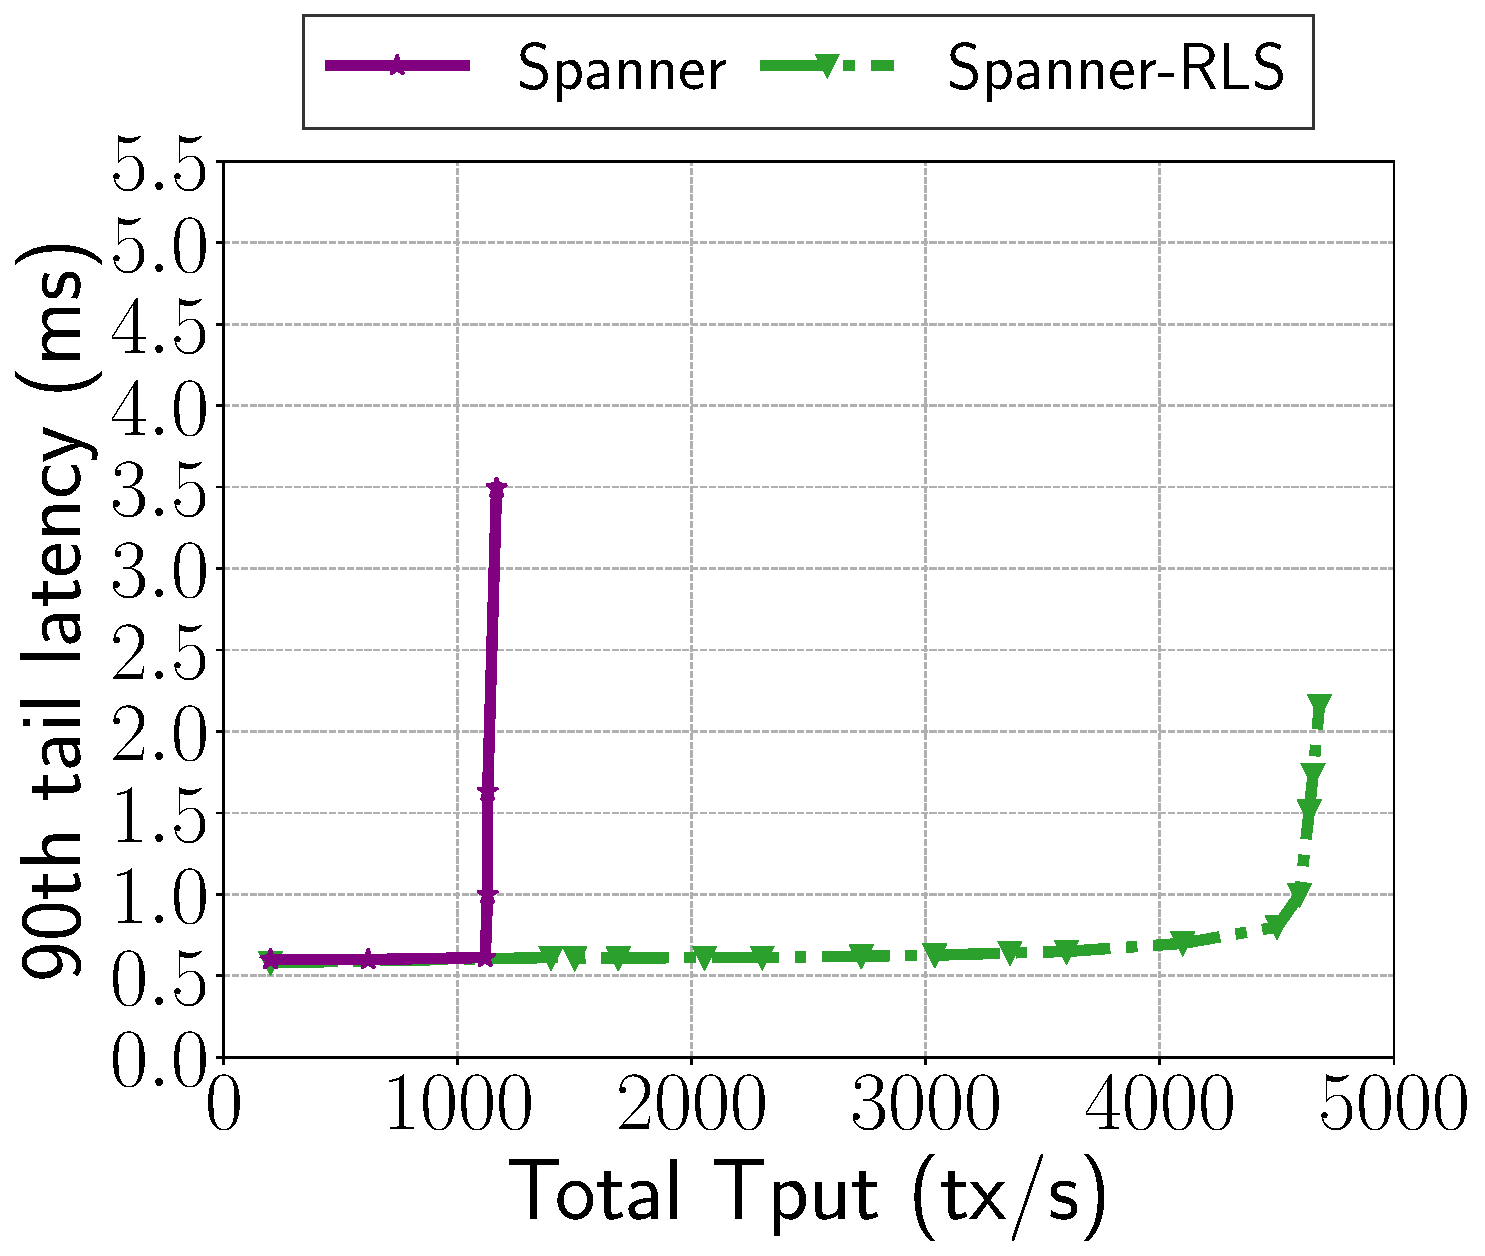
\includegraphics[width=0.45\columnwidth]{eval-figs/spanner_lat_tput_waitdie.pdf}
	}
	\hfill
	\subfloat[\footnotesize Tail latency.\label{fig:spanner:overview:wait:breakdown}]{
		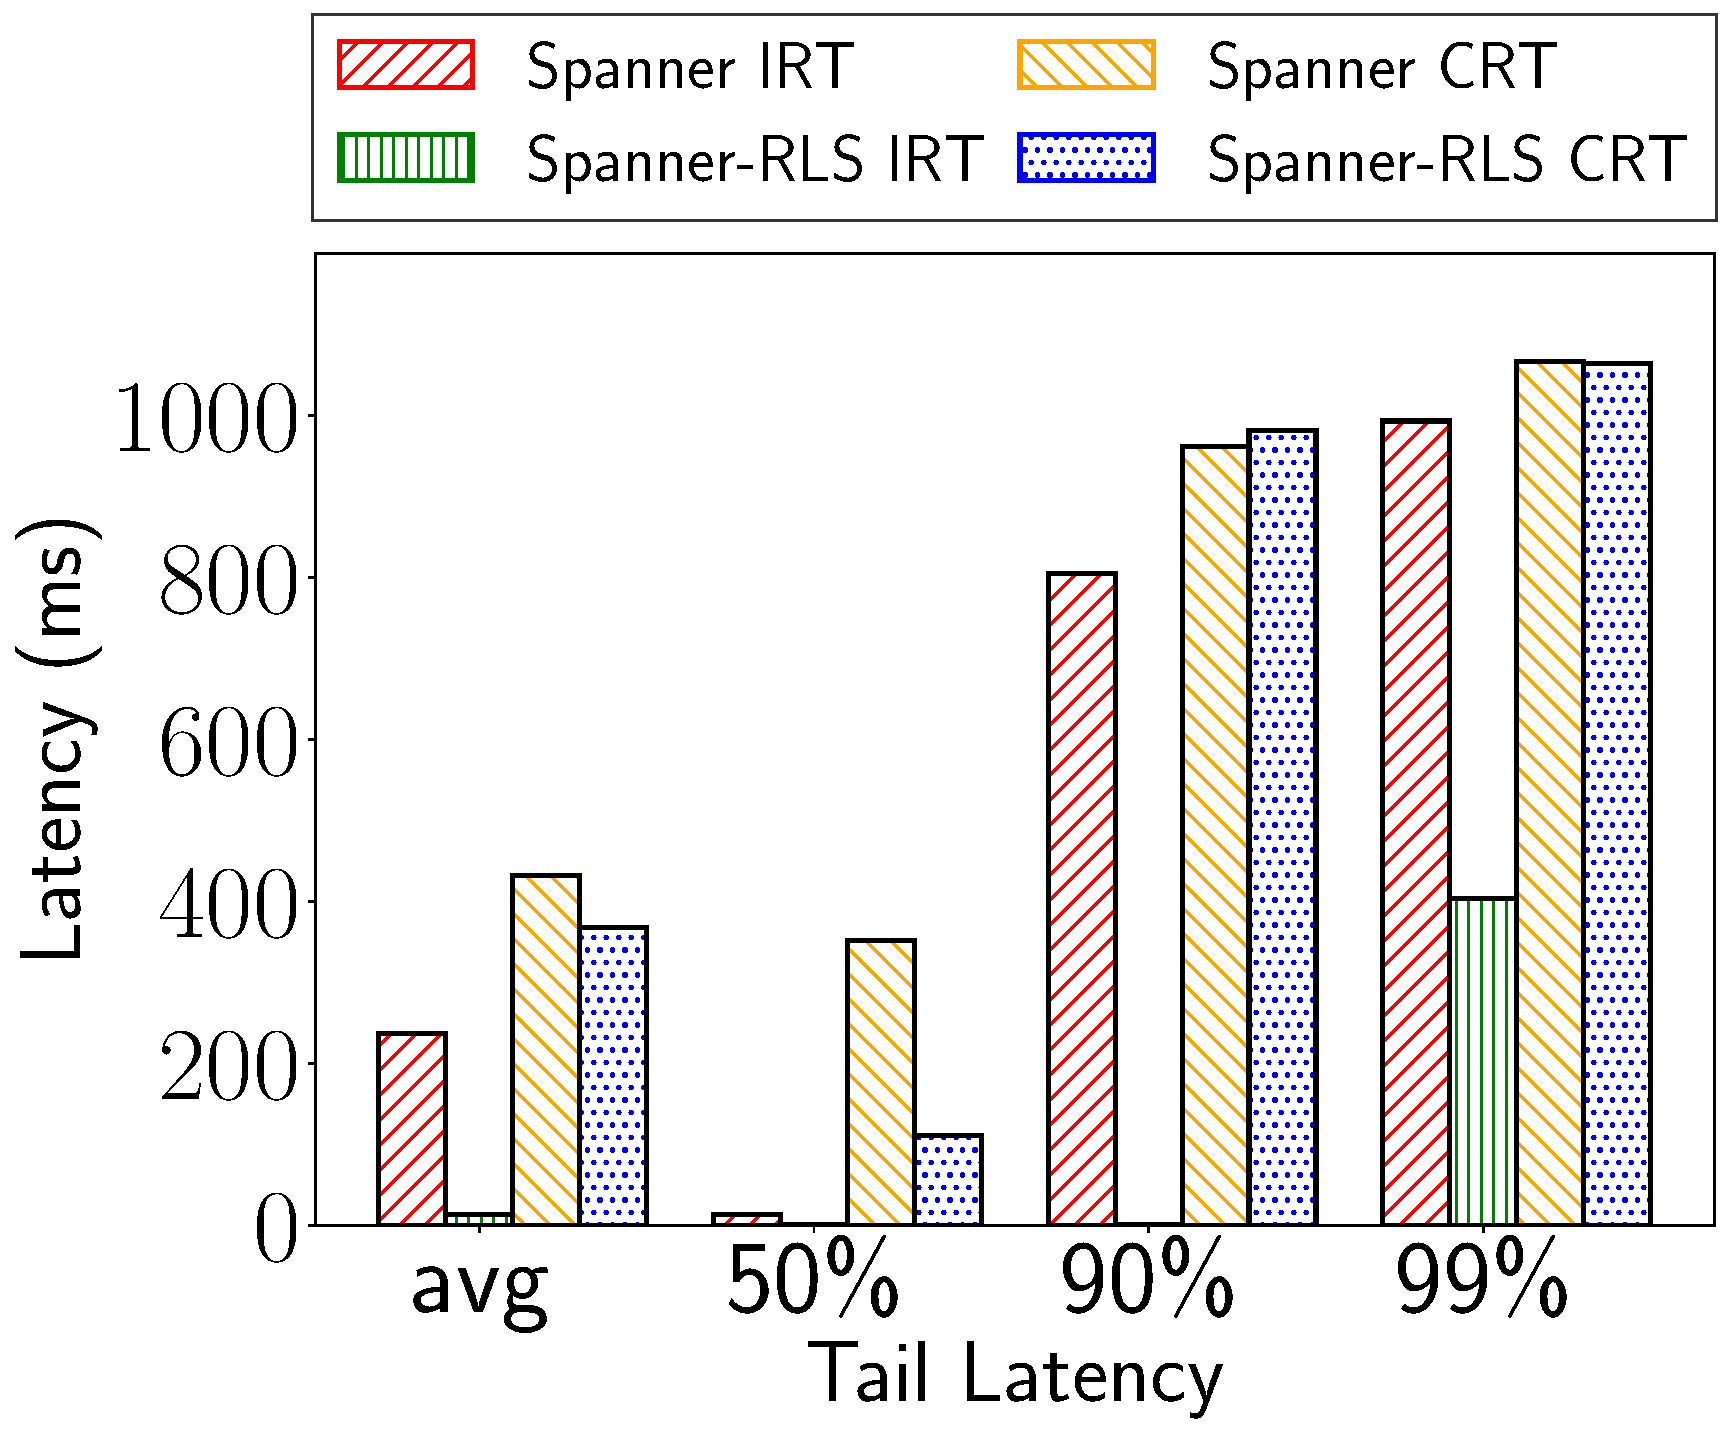
\includegraphics[width=0.45\columnwidth]{eval-figs/spanner_abortrate.pdf}
	}
	\caption{Overall performance and latency of Spanner and Spanner-RLS  on YCSB-T (default setting) using \texttt{WAIT\_DIE}.}\label{fig:eval:spanner:overall:wait}
\end{figure}


\begin{figure*}[t]
	\centering
	
\includegraphics[width=2\columnwidth]{eval-figs/legend_Spanner.png}
	\vspace{1pt}
	\subfloat[\footnotesize Impact of Concurrency\label{fig:spanner:concurrency:abort}]{
		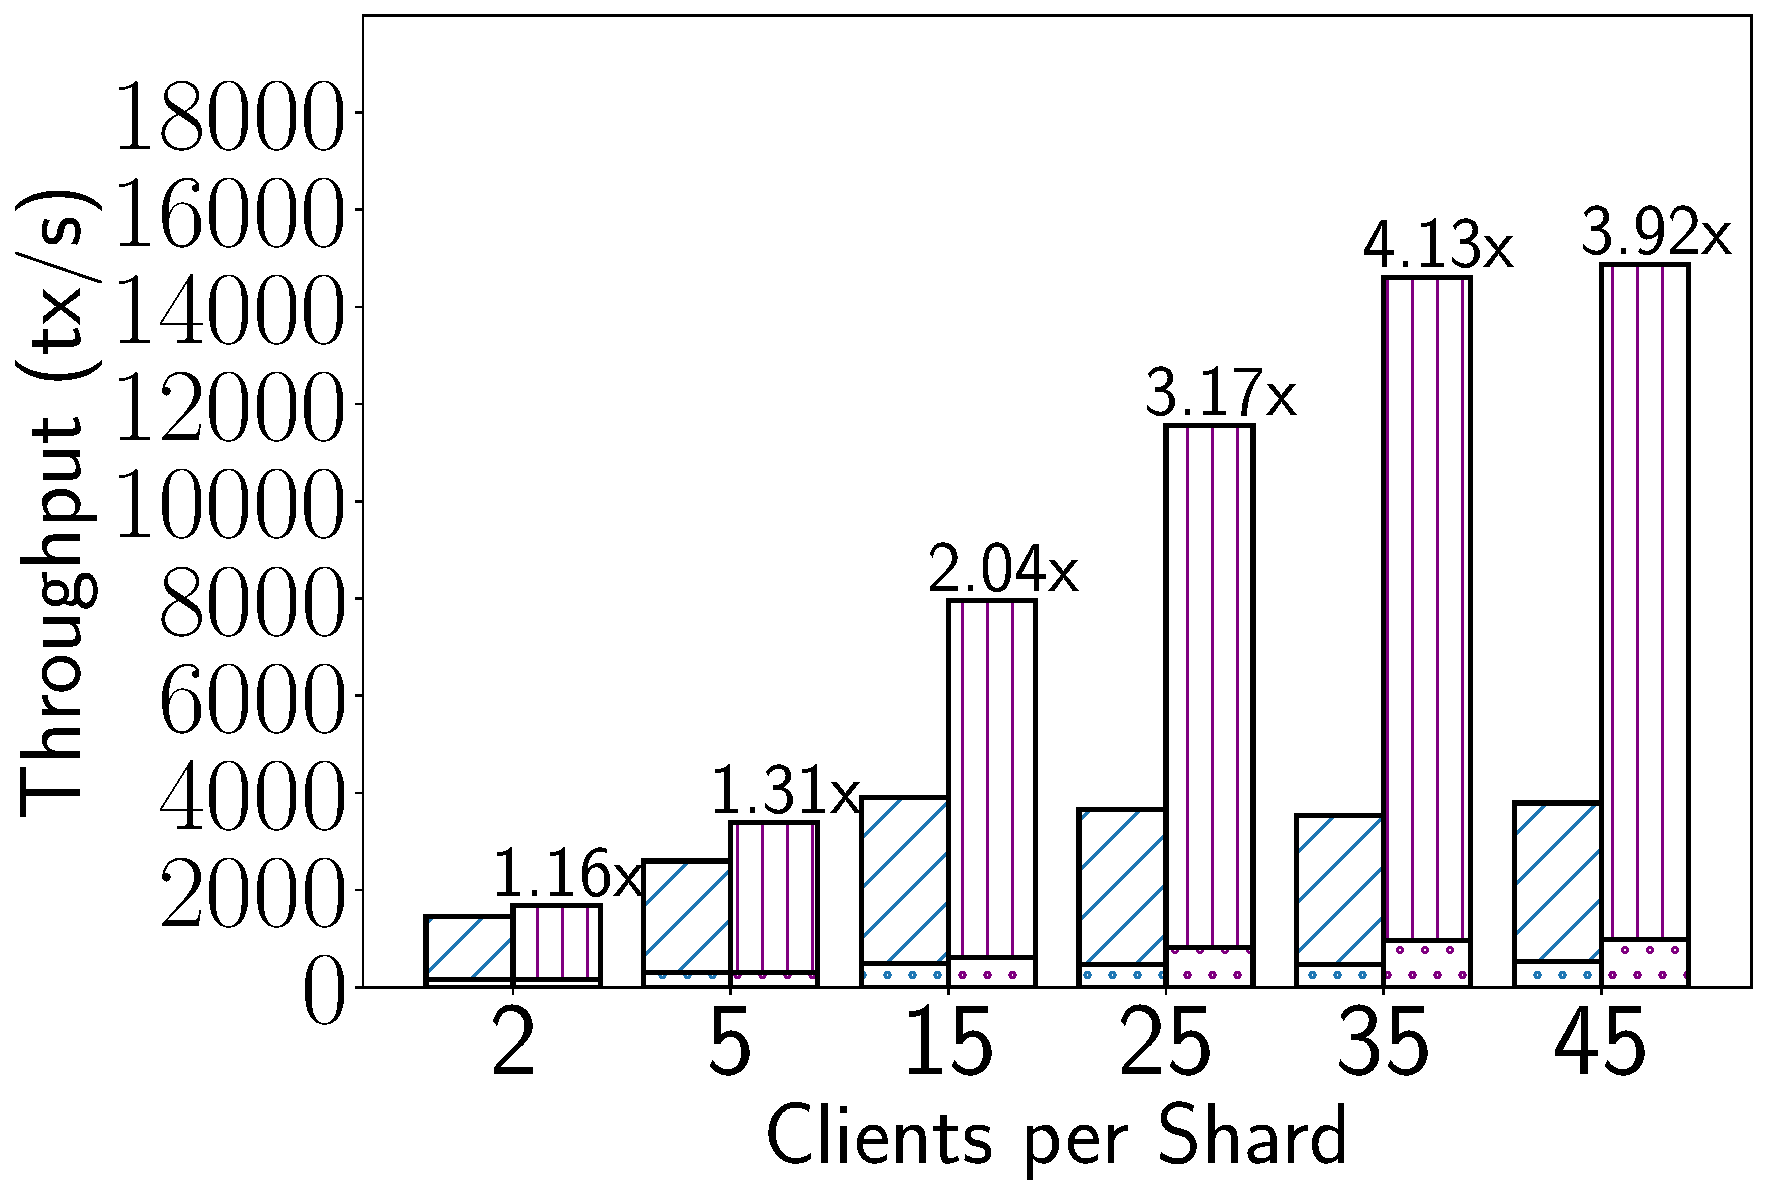
\includegraphics[width=0.48\columnwidth]{eval-figs/spanner_tput_client.pdf}
	}
	\hfill
	\subfloat[\footnotesize Impact of CRT\label{fig:spanner:crt:abort}]{
 	    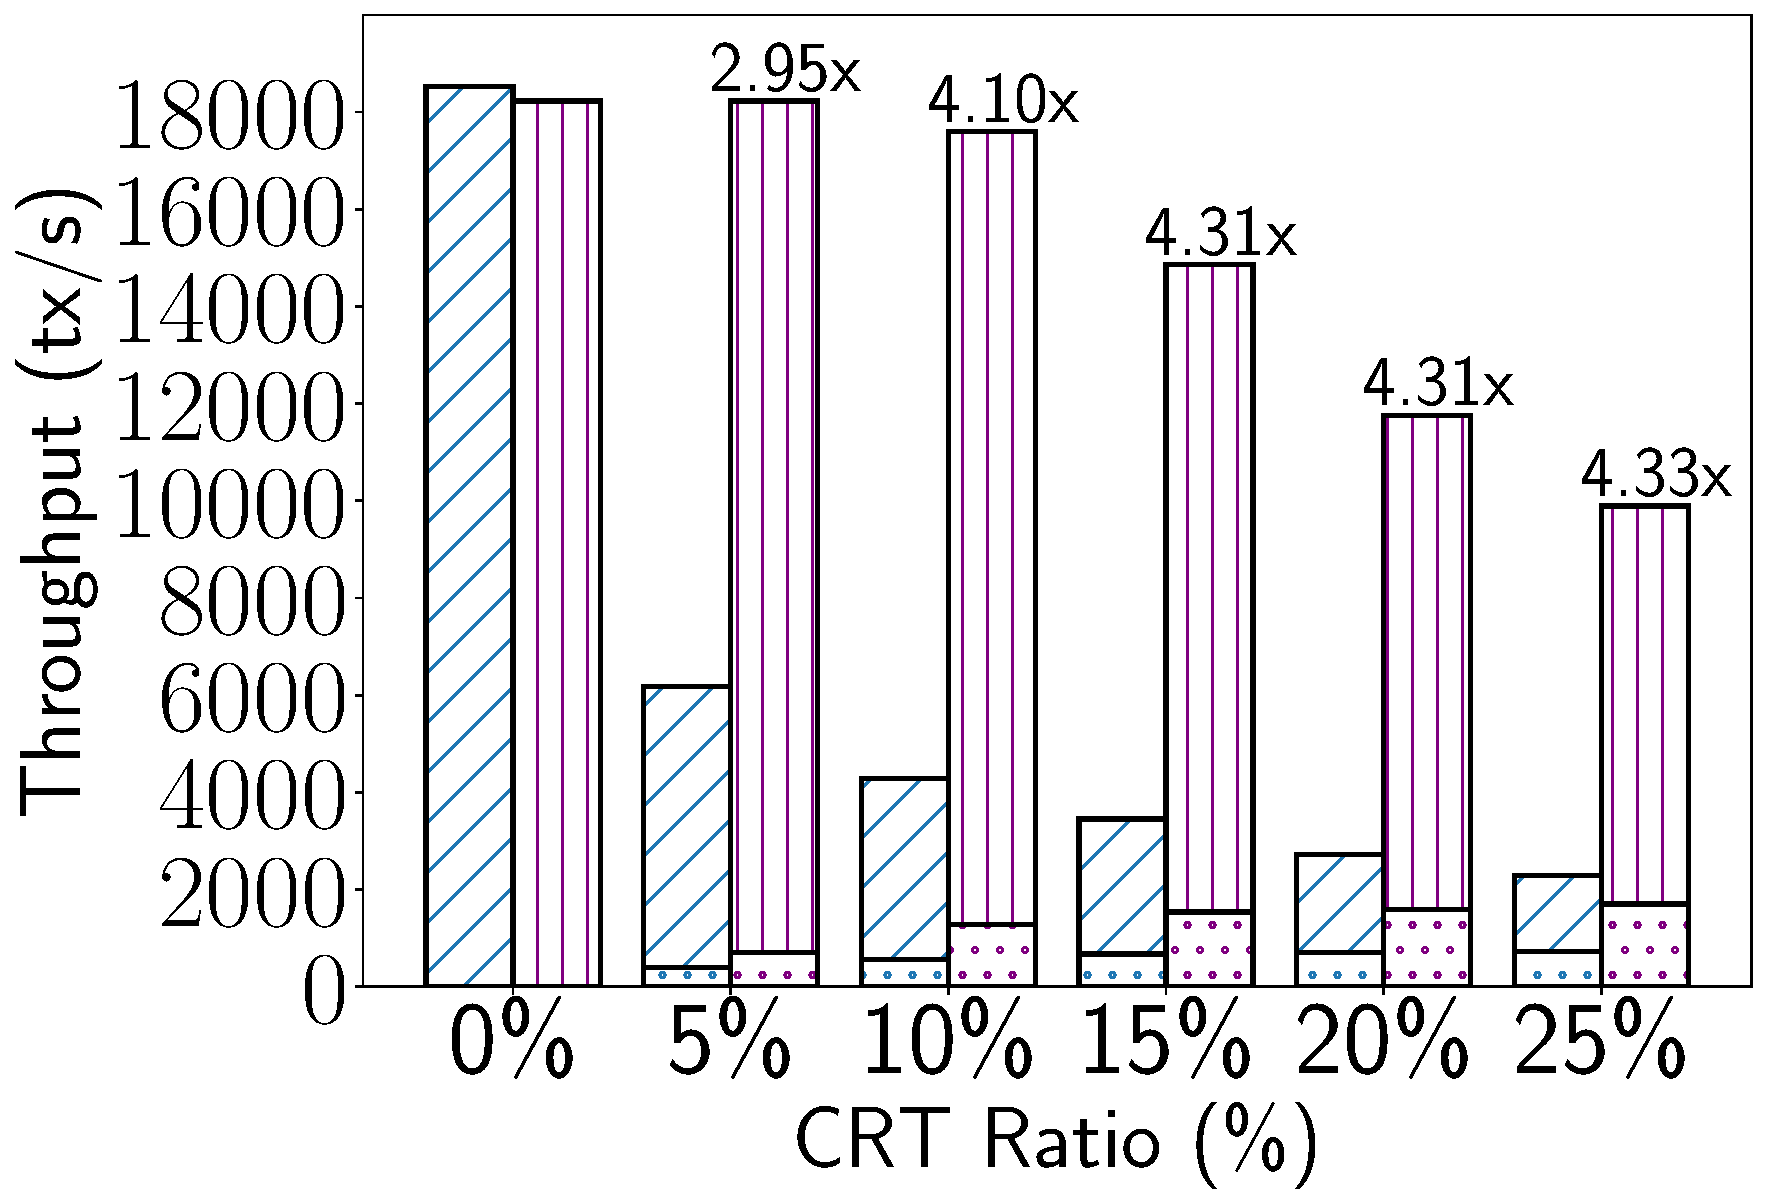
\includegraphics[width=0.48\columnwidth]{eval-figs/spanner_tput_crt.pdf}
	}
	\hfill
	\subfloat[\footnotesize Impact of RTT\label{fig:spanner:rtt:abort}]{
  	   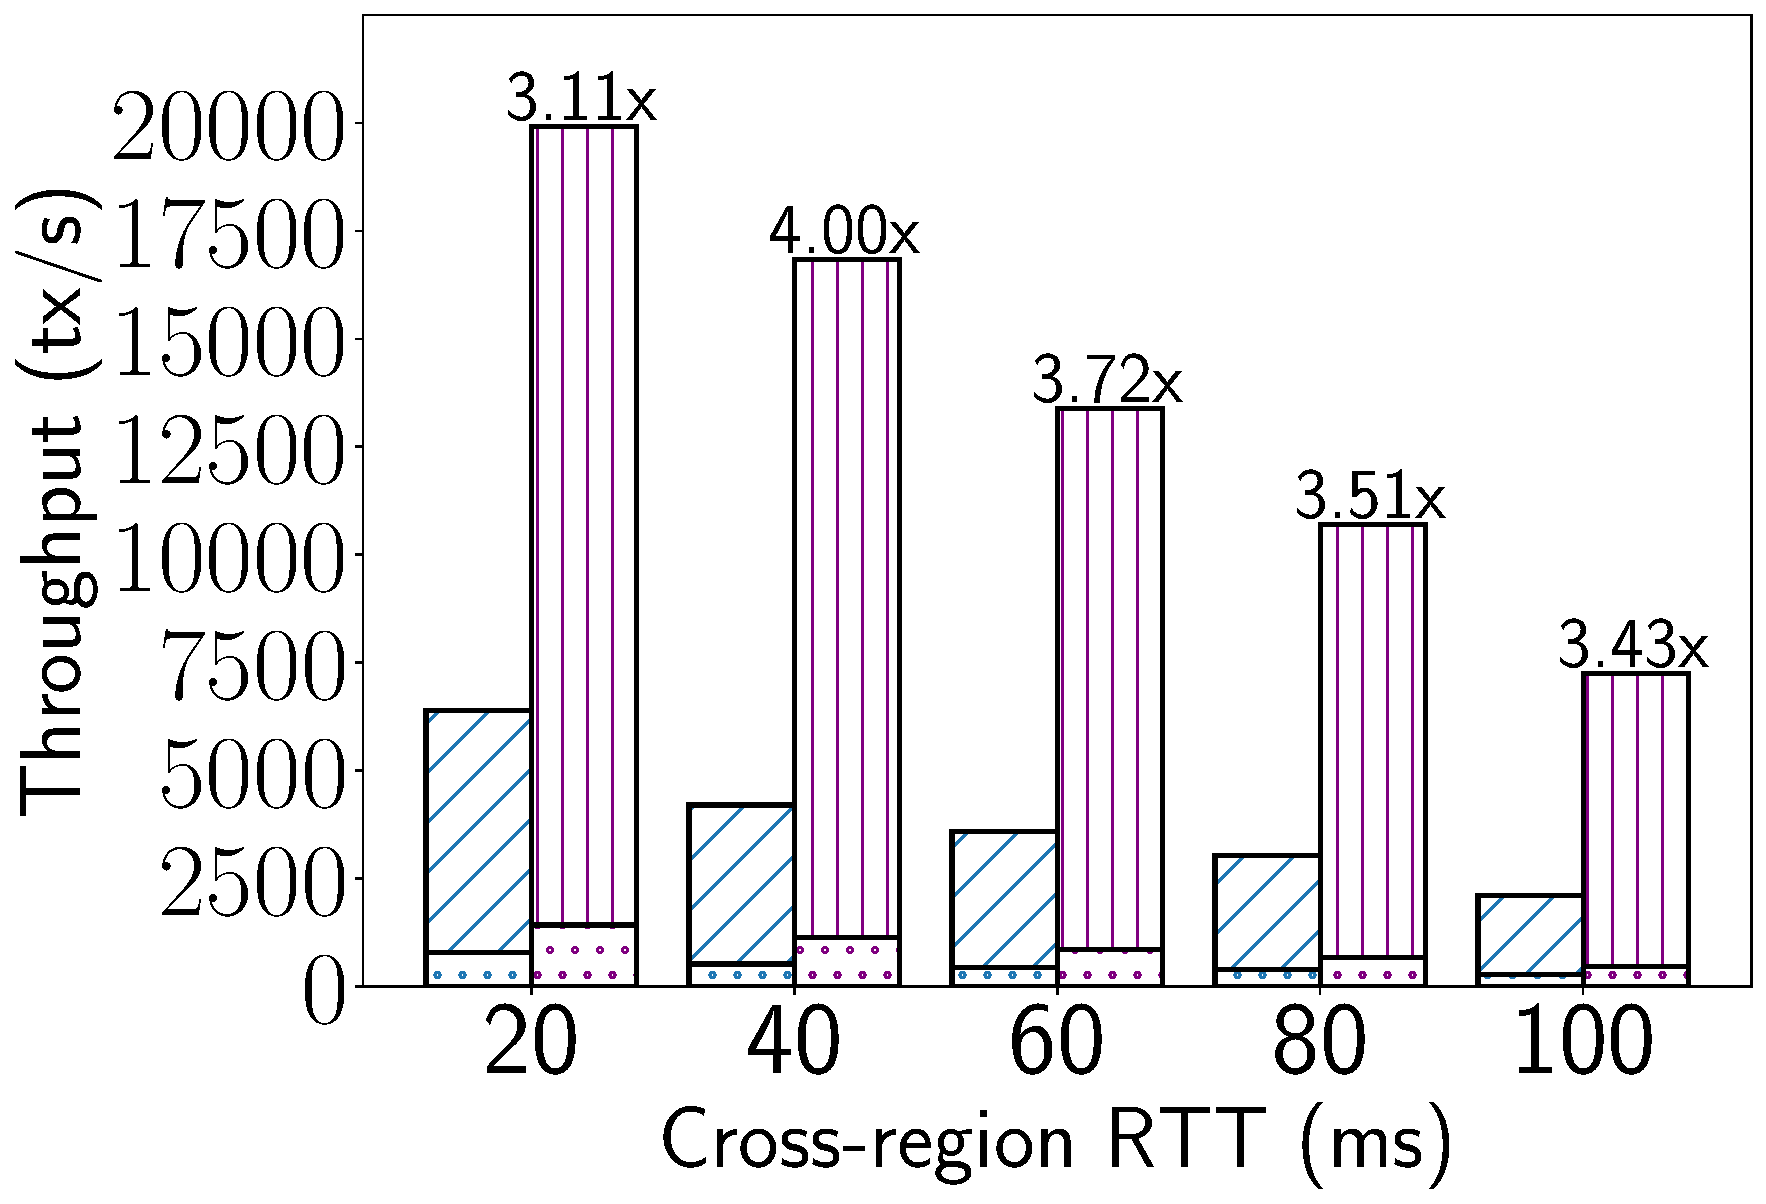
\includegraphics[width=0.48\columnwidth]{eval-figs/spanner_tput_rtt.pdf}
	}
	\hfill
	\subfloat[\footnotesize Impact of Conflicts\label{fig:spanner:zipf:abort}]{
        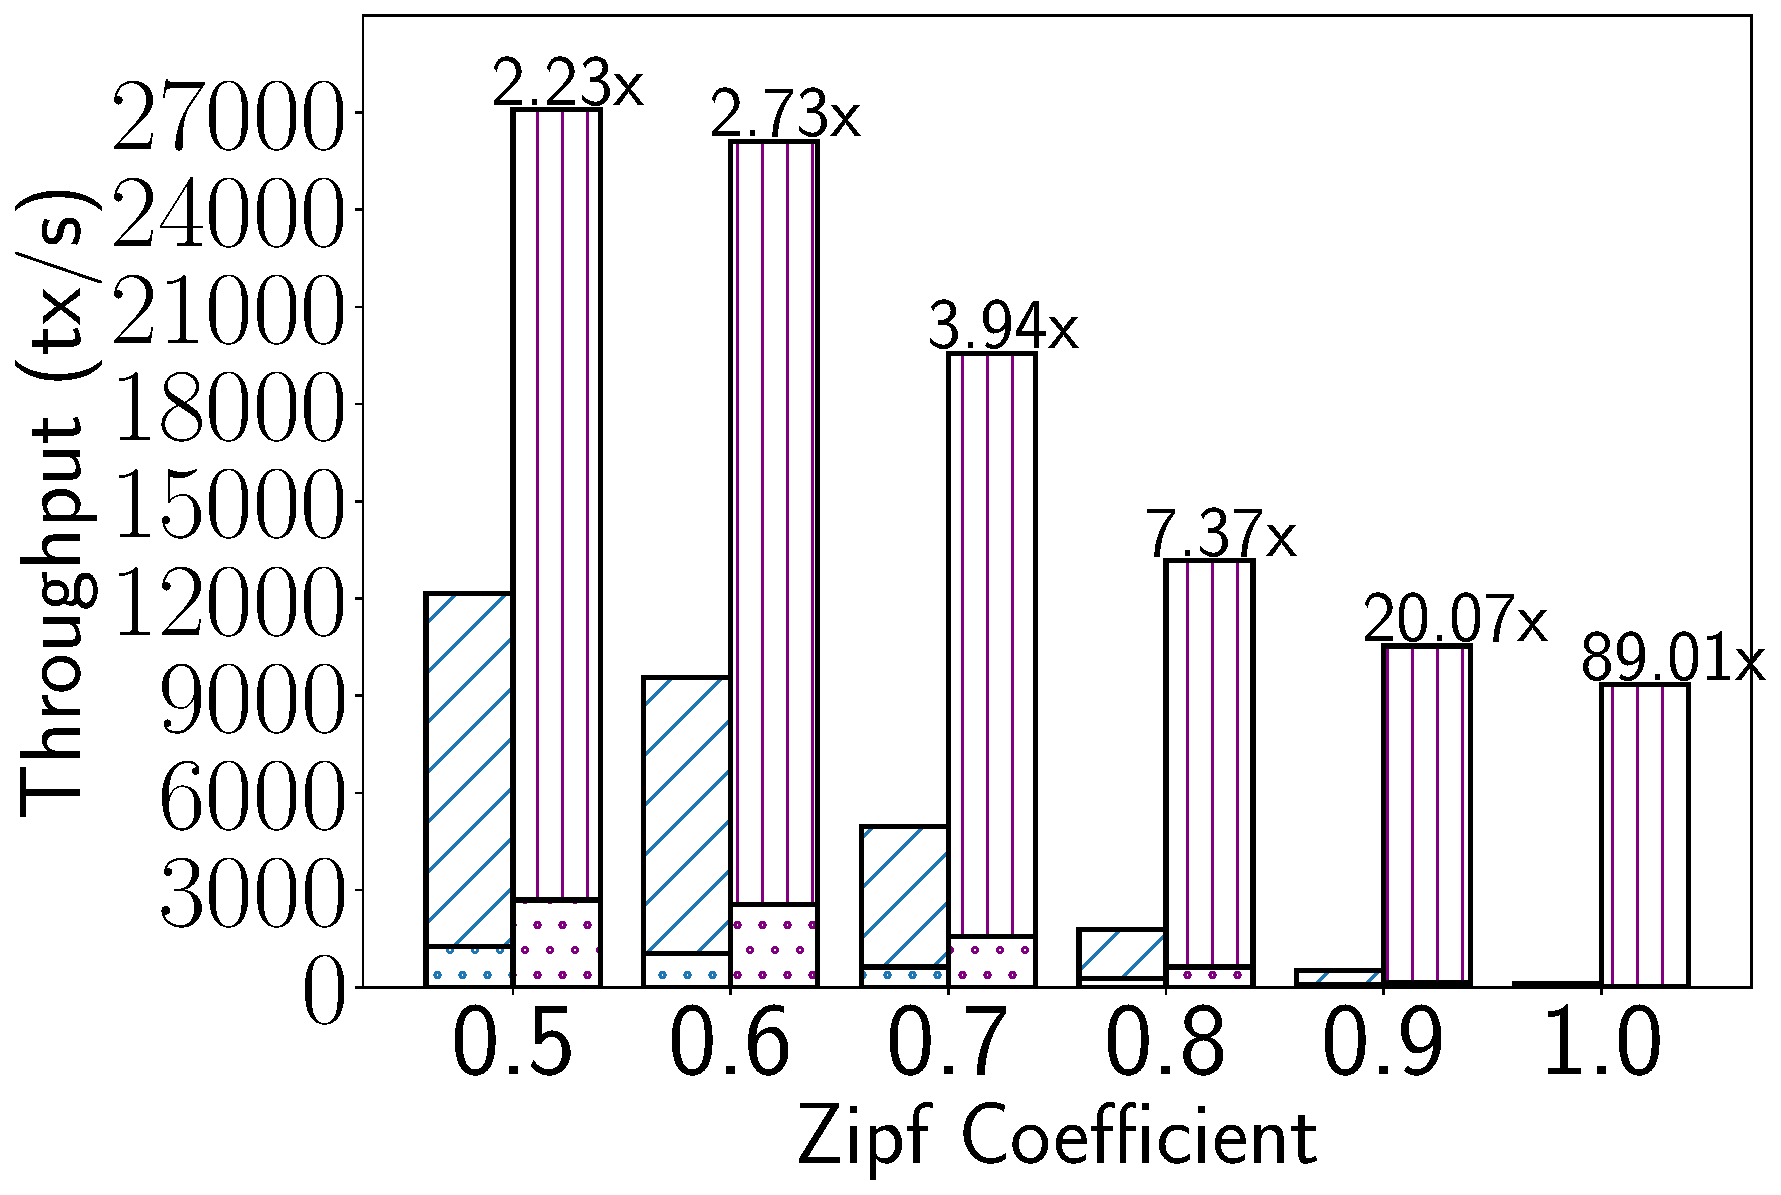
\includegraphics[width=0.48\columnwidth]{eval-figs/spanner_tput_zipf.pdf}
	}

	\caption{Performance of Spanner and Spanner-RLS on YCSB-T with different experimental parameters using \texttt{NO\_WAIT}.}\label{fig:eval:spanner:abort}
% \vspace{10pt}
\end{figure*}

\begin{figure*}[t]
	\centering
	
\includegraphics[width=2\columnwidth]{eval-figs/legend_Spanner.png}
	\vspace{1pt}
	\subfloat[\footnotesize Impact of Concurrency\label{fig:spanner:concurrency:wait}]{
		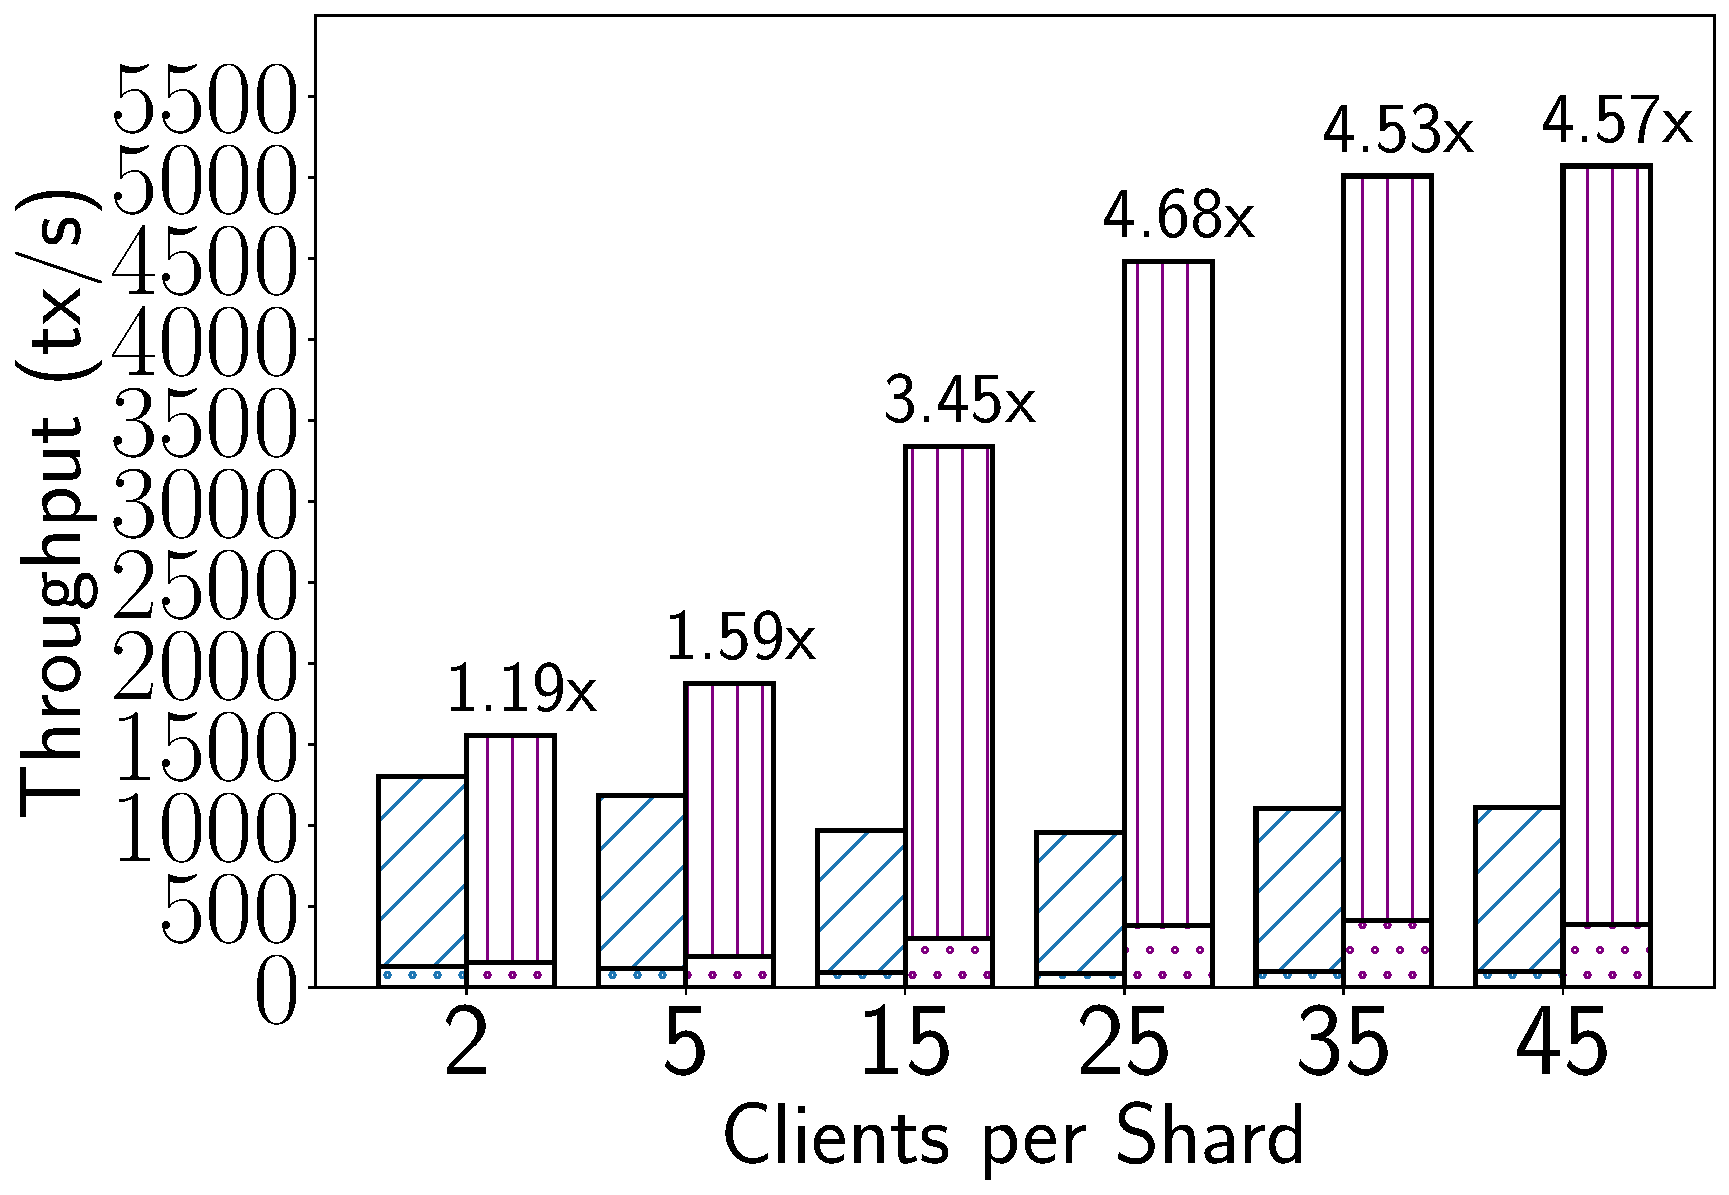
\includegraphics[width=0.23\textwidth]{eval-figs/spanner_tput_client_waitdie.pdf}
	}
	\hfill
	\subfloat[\footnotesize Impact of CRT\label{fig:spanner:crt:wait}]{
 	    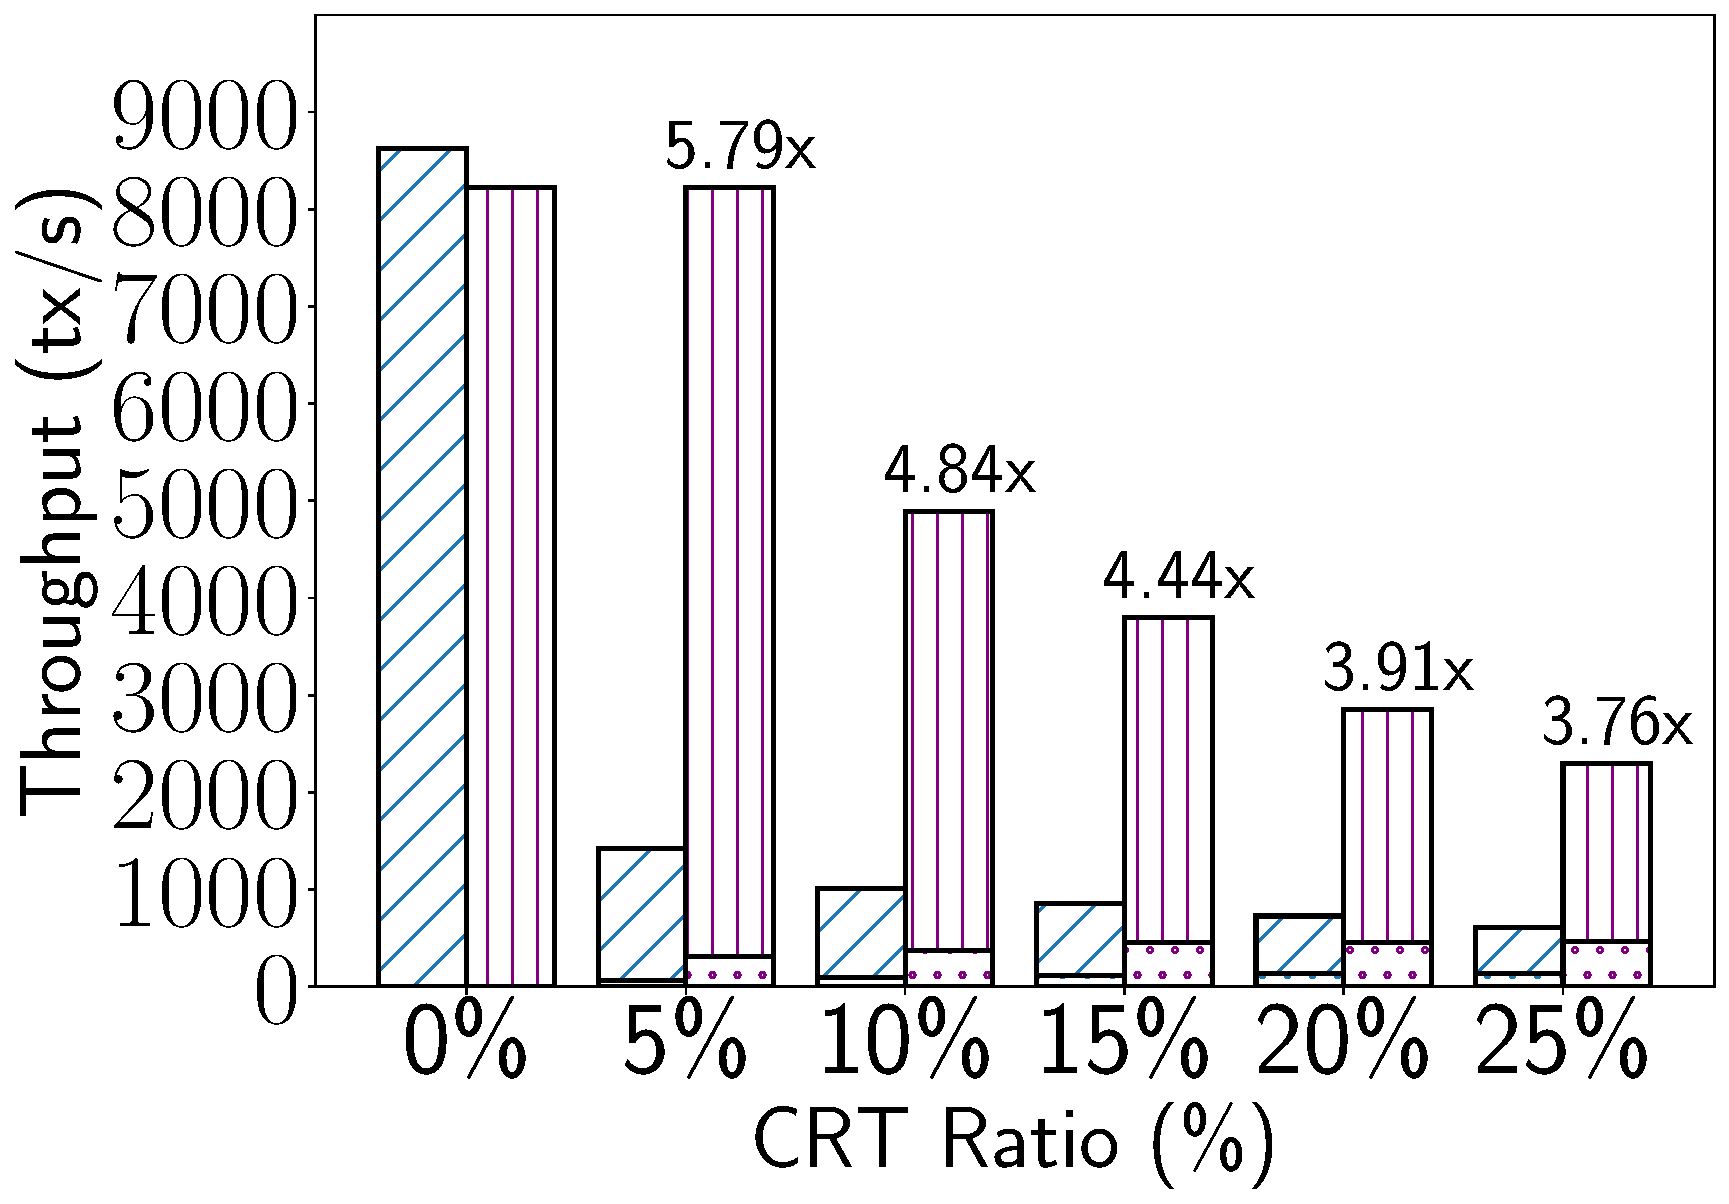
\includegraphics[width=0.23\textwidth]{eval-figs/spanner_tput_crt_waitdie.pdf}
	}
	\hfill
	\subfloat[\footnotesize Impact of RTT\label{fig:spanner:rtt:wait}]{
  	   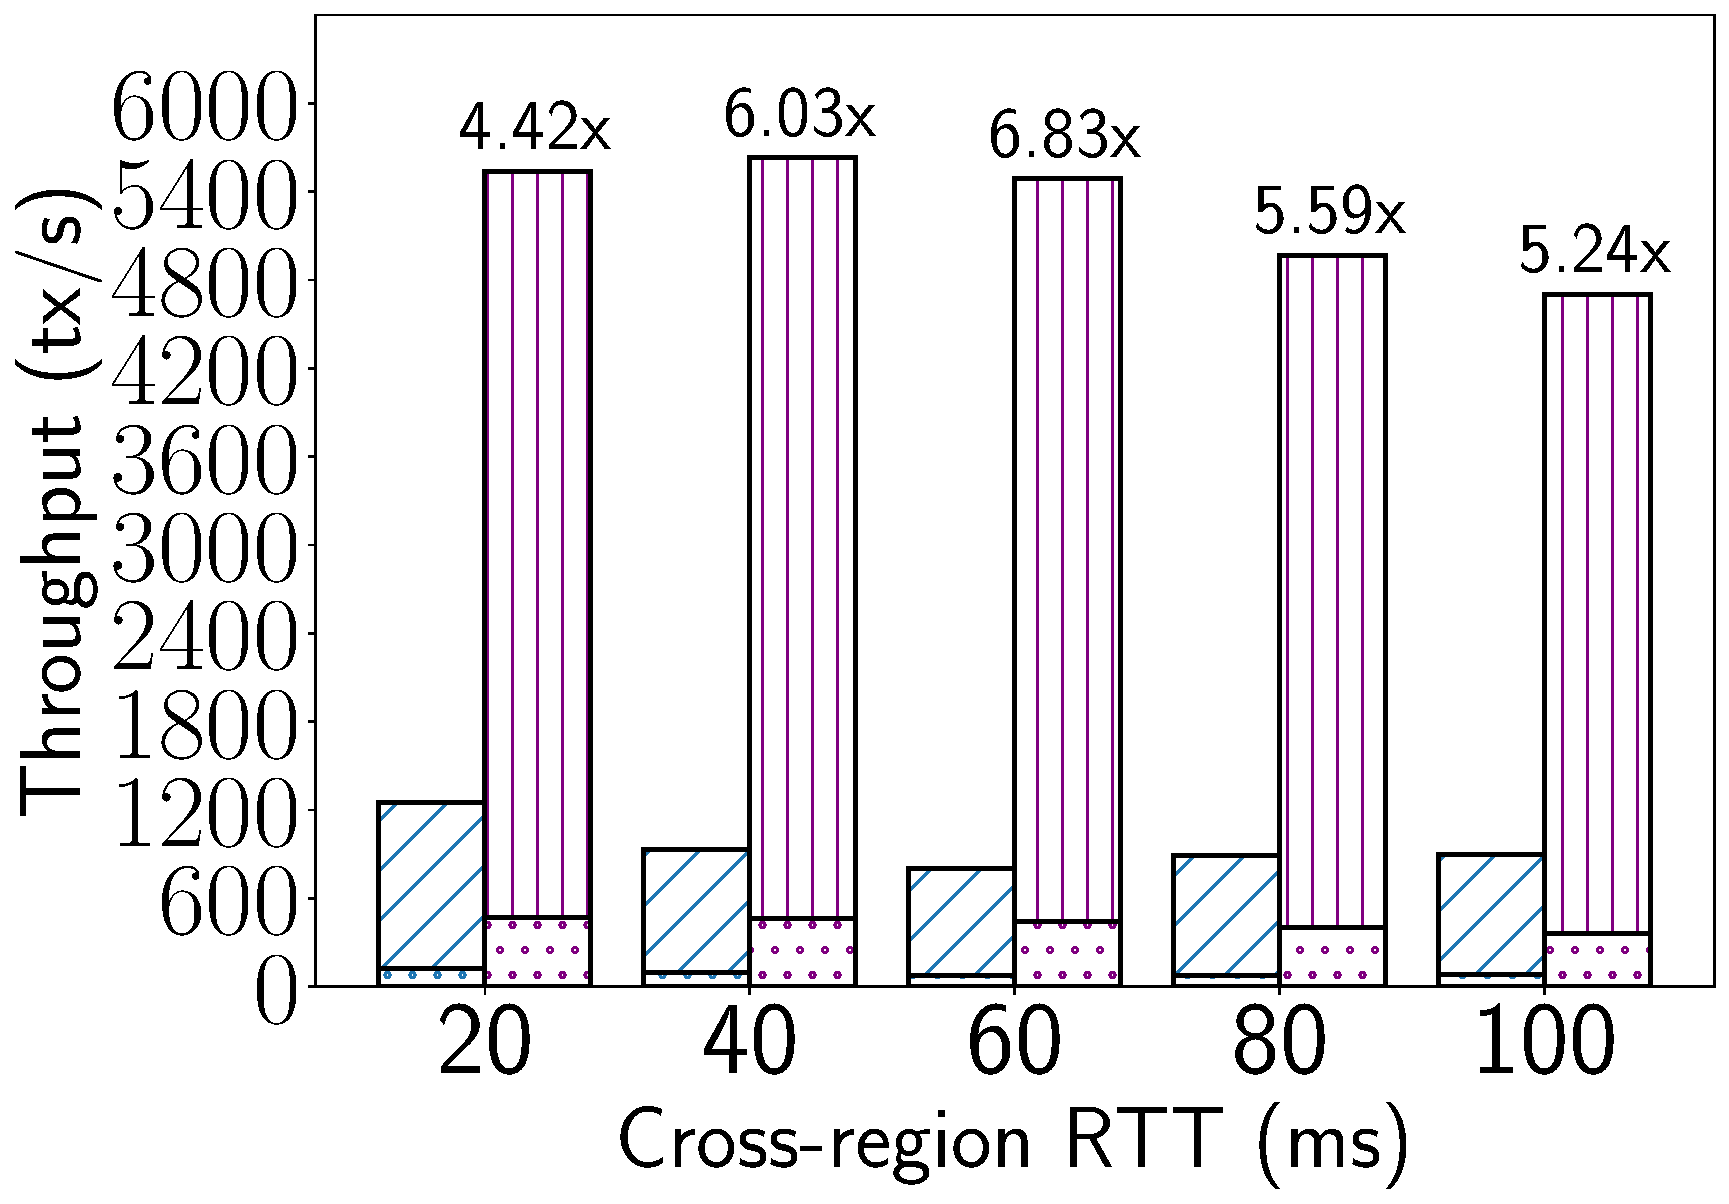
\includegraphics[width=0.23\textwidth]{eval-figs/spanner_tput_rtt_waitdie.pdf}
	}
	\hfill
	\subfloat[\footnotesize Impact of Conflicts\label{fig:spanner:zipf:wait}]{
        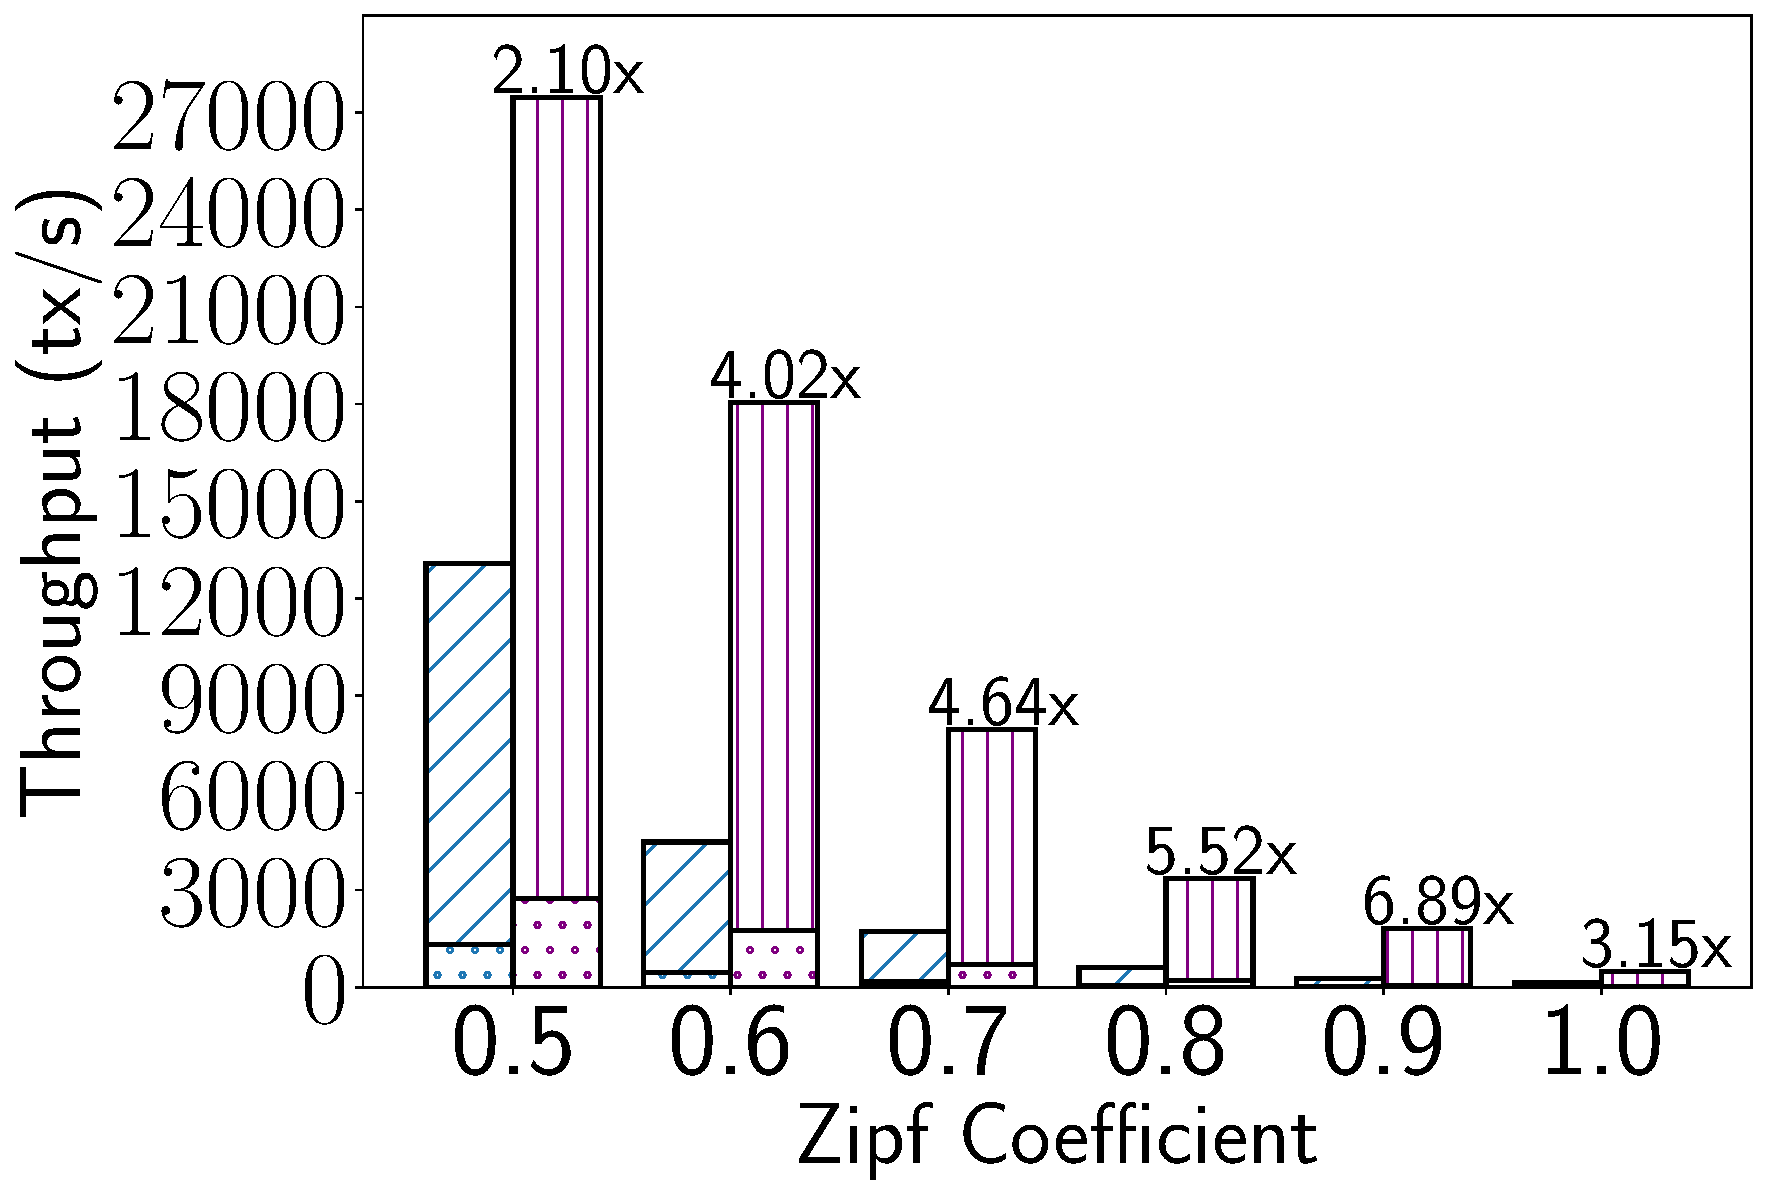
\includegraphics[width=0.23\textwidth]{eval-figs/spanner_tput_zipf_waitdie.pdf}
	}
  
	\caption{Performance of Spanner and Spanner-RLS on YCSB-T with different experimental parameters using \texttt{WAIT\_DIE}.}\label{fig:eval:spanner:wait}
	\vspace{10pt}
\end{figure*}

\begin{itemize}[leftmargin=*, itemsep=1.5pt]
    \setlength{\itemsep}{0pt}
    \setlength{\parsep}{0pt}
    \setlength{\parskip}{0pt}
\item \textbf{\texttt{NO\_WAIT.}} When using this deadlock mechanism, if a lock request is denied, the database will immediately abort the requesting transaction, and the client will retire the transaction. 
\item \textbf{\texttt{WAIT\_DIE.}} Unlike \texttt{NO\_WAIT}, \texttt{WAIT\_DIE} allows a transaction to wait for the requested lock if the transaction is older than the one that holds the lock. Otherwise, the transaction is forced to abort and will be retired by the client. 
\end{itemize}

We do not consider other deadlock mechanisms since they are either subsumed by the two mechanisms or will incur significant overhead in a multi-region deployment. 
For instance, deadlock detection necessitates a centralized deadlock detector for cycle detection, which can be expensive due to cross-region communication.

\subsubsection{Performance Overview} 

We first evaluated the performance under the default setting. For an apple-to-apple comparison, we refrained from using prior knowledge of read and write sets in our experiments, even though the read and compose set of YCSB-T can be revealed before execution. As shown in \fig{fig:spanner:overview:abort}  and \fig{fig:spanner:overview:wait}, Spanner-RLS significantly outperformed Spanner on YCSB-T. In particular, Spanner-RLS achieved $3.95\times$ and $4.27\times$ higher peak throughput when utilizing \texttt{NO\_WAIT} and \texttt{WAIT\_DIE}, respectively. Spanner-RLS's $90th$ resembled that of Spanner, essentially representing the IRTs latency. We observed that employing the \texttt{NO\_WAIT} mechanism resulted in substantially higher throughput than using \texttt{WAIT\_DIE}, given the default workload's write-intensive nature with medium contention.

To comprehend how our new design contributes to performance improvement, we gathered data on the abort rate for \texttt{NO\_WAIT} and tail latency for \texttt{WAIT\_DIE} when both Spanner and Spanner-RLS achieved the peak throughput. \fig{fig:spanner:overview:abort:breakdown} and \fig{fig:spanner:overview:wait:breakdown} illustrate the results. 

Regarding \texttt{NO\_WAIT}, Spanner-RLS can efficiently reduce the abort rate for both IRTs and CRTs. The overall abort ratedecreased from $56\%$ to $33\%$ (i.e., $41.1\%$ reduction). In particular, Spanner-RLS achieved a  more significant reduction for IRTs (from $40\%$ to $6\%$) due to the ``non-blocking'' property in IRT coordination and commitment. It's worth mentioning that the $6\%$ abort rate was only caused by the contention among IRTs. Meanwhile, the abort rate of CRTs also saw a reduction. However, compared to IRTs, CRTs still exhibited a much higher abort rate (i.e., $27.42\%$) due to the larger contention footprint.

For \texttt{WAIT\_DIE}, Spanner-RLS achieved a significantly lower average latency for IRTs, while the average latency of CRTs was roughly the same as in Spanner. This is attributed to the fact that in Spanner-RLS, an IRT will never be blocked by CRTs. The results on $50th$ and $90th$ latency support this assertion. Both Spanner and Spanner-RLS exhibited low $50th$ latency, while the $90th$ latency of Spanner and Spanner-RLS was $805ms$ and $1.4ms$, respectively. The $99th$ latency of Spanner-RLS increased due to the queueing effect in the software stack. 

Next, we delve into understanding how Spanner-RLS and Spanner are affected by various workload parameters. These experiments were conducted using YCSB's APIs as they offer flexibility in configuration.



\subsubsection{Impact of Concurrency} We first compare the performance of Spanner-RLS and Spanner under various concurrencies. As illustrated in \fig{fig:spanner:concurrency:abort} and \fig{fig:spanner:concurrency:wait}, Spanner's throughput reached saturation rapidly as the number of clients increased. Consequently, the peak throughput of Spanner was $3911$ and $1181$ transactions per second using \texttt{No\_WAIT} and \texttt{WAIT\_DIE}, respectively. In contrast, Spanner-RLS could serve more clients and achieve a substantially higher peak throughput.

\subsubsection{Impact of CRT Ratio} We studied the impact of the CRT ratio by fine-tuning the workload generation. As shown in \fig{fig:spanner:crt:abort} and \fig{fig:spanner:crt:wait}, when CRTs were enabled, Spanner experienced 
severe performance degradation (e.g., throughput dropping from $18526$ transactions per second to $6184$ transactions per second when the CRT ratio increased from $0\%$ to $5\%$), aligning with our discussion in \chref{sec:intro} and \chref{sec:background:geo}. In contrast, Spanner-RLS's performance degraded slightly, attributed to the elimination of cross-region costs for IRTs. In scenarios where all transactions were IRTs (i.e., a special case in our experiments), Spanner-RLS demonstrated slightly lower throughput than Spanner due to the cost for extra steps in concurrency control (i.e., checking transaction types even if all transactions are IRTs). With a continuous increase in CRT ratios, the throughput of Spanner and Spanner-RLS decreased due to cross-region communication costs. In practice, the CRT ratio of workloads should not be too high since the cost of CRT itself is still relatively high compared to IRTs. Real-world workloads show good data locality under multi-region deployment (\chref{sec:background:deployment}), facilitating low-latency data access.



\subsubsection{Impact of Cross-Region RTT} Next, we studied the impact of the cross-region network delays, a critical factor affecting the overall cost of CRTs. Larger cross-region network delays generally result in longer transaction coordination and commit times for CRTs. The results, illustrated in \fig{fig:spanner:rtt:abort} and \fig{fig:spanner:rtt:wait}, clearly indicate that Spanner-RLS outperforms Spanner regardless of the cross-region network delays. In fact, Spanner-RLS demonstrates more when the network delays are moderate (e.g., $40s$ and $60s$ for a cross-region network round trip). In addition, the network delay amplifies the advantages of Spanner-RLS while also affecting Spanner-RLS's CRTs, causing a drop in throughput from $1429$ transactions per second to $476$ transactions per second as the network delay increased from $20$ seconds to $100$ seconds using \texttt{NO\_WAIT}.



\subsubsection{Impact of Contention} In our final experiment, we compared the performance under various contention by adjusting the skewness of Zipf distribution in YCSB-T while keeping other parameters consistent with the default settings. The results depicted in \fig{fig:spanner:zipf:abort} and \fig{fig:spanner:zipf:wait} consistently show that the Spanner-RLS's throughput outperforms Spanner's across all levels of contention. This improvement stems from Spanner-RLS efficiently reducing the contention footprint by ordering IRTs and CRTs independently. As discussed in \chref{sec:background:geo}, the contention footprint of IRTs eliminates both ``coordination blocking'' and ``commit blocking'', which is extremely expensive in multi-region deployments. As expected by our analysis, Spanner-RLS gained larger margins under high contention. This is because, under high contention, IRTs in Spanner have more chance to be blocked by CRTs, leading to poor performance. It should be noted that the performance of Spanner-RLS also degraded due to the cost of acquiring locks, and \texttt{NO\_WAIT} consistently outperformed \texttt{WAIT\_DIE} since \texttt{WAIT\_DIE} suffers more from lock thrashing and timestamp allocation when the contention is higher.

\subsection{Takeaways}
By adhering to the principles of RLS, developers can significantly enhance the performance of Spanner. Spanner-RLS serves as a practical example, illustrating how RLS can assist multi-region databases in achieving an optimal balance between consistency and performance. Further enhancements in the performance of Spanner-RLS can be achieved by implementing advanced optimizations (e.g., a pre-write-log mechanism in RedT~\cite{zhang2023redt}), which is orthogonal to our paper. We believe our study on Spanner-RLS holds the potential to guide future research by encouraging researchers and developers to consider multi-level two-phase locking and two-phase commit. Even though the design of Spanner-RLS may not be directly applicable to other strictly serializable concurrency protocols due to potential differences in transaction coordination mechanisms, the fundamental concept of RLS remains applicable.



\section{\crdb and \crdbxx}\label{sec:crdb}
This section presents the design, implementation, and evaluation of Cockroachdb (for short, CRDB) and CRDB-RLS. We show that RLS has the potential to evolve the consistency model of existing databases (i.e., providing tighter and stronger consistency guarantees) without sacrificing performance. 

\subsection{Protocols and Implementations}

\noindent\textbf{CRDB Background.} CRDB~\cite{taft2020cockroachdb} is an open-source production-grade database system that began as an external Spanner clone. Like Spanner, CRDB aims to build a resilient geo-distributed SQL Database with serializable ACID transactions.

Overall, \crdb provides single-key linearizability (i.e., no stale reads for each key) by supporting multi-version timestamp ordering (MVTO). The transaction manager nodes in CRDB are the special nodes for interacting with clients, assigning timestamps to transactions, and driving transaction coordination. CRDB assumes a maximum clock offset among transaction managers (i.e., using $500ms$ by default), which is critical to its correctness.

\crdb's consistency model (i.e., single-key linearizability) is strictly weaker than \xxcons as \crdb ensures only a subset of \xxcons's guarantees: \crdb does not preserve the real-time ordering for any pair of non-conflicting transactions, while RLS provides real-time order among IRTs in the same region. We refer readers to \chref{sec:rls:compare} for detailed comparisons between RLS and Single-Key Linearizability (SKL). 

\newcommand\mycommfont[1]{\footnotesize\sffamily\textcolor{red}{#1}}
\SetCommentSty{mycommfont}
\SetKwProg{Fn}{function}{:}{}

\SetKwFunction{FMax}{max}
\SetKwFunction{FNow}{now}
\SetKwFunction{Coordcr}{CRDB-RLS Coordinator}
\SetKwFunction{FGetFinTs}{GetFinishedTs}
\SetKwFunction{FVerifyReads}{VerifyReads}
\SetKwFunction{Leader}{GetShardLeader}
\SetKwFunction{FSend}{send}
\SetKwFunction{FKeyLeader}{keyLeader}

\SetKwData{InFlightOps}{inflightOps}
\SetKwData{TouchedR}{touchedRegions}
\SetKwData{TxnTs}{txnTS}
\SetKwData{DOp}{op}
\SetKwData{DRegion}{r}
\SetKwData{DResp}{resp}

\begin{algorithm}[t]
    \setstretch{1}
    \small
    % \LeftComment{Execute the transaction commands, which triggers the events:}
    \Fn{\Coordcr}{
      \InFlightOps $\gets \emptyset$   \Comment{Ongoing operations.} \\
      \TouchedR $\gets \emptyset$  \Comment{Regions involved in the transaction.} \\
      \TxnTs $\gets$ \FNow{}   \Comment{Timestamp of the transaction.} \\

      \For{\DOp $\gets$ KV operation received from SQL layer}{
        \uIf{\DOp.commit}{
          \DOp.deps $\gets$ \InFlightOps \\
          \FSend $\langle \texttt{commit}, \TxnTs \rangle$ to transaction managers \\
          wait for all \texttt{ACK}s \\
        }
        \Else(){
          % \tcp{New in \crdbxx}
          \tikzmk{A}
          \DRegion $\gets$ \DOp.key.region \\
          \If{$\DRegion \notin \TouchedR$}{
            \TxnTs $\gets$ \FMax{\TxnTs, \FGetFinTs{\DRegion}} \\
            \FVerifyReads{\TxnTs} \\
            \TouchedR $\gets$ \TouchedR $\cup$ \{\DRegion\} \\
          }
          \tikzmk{B} \boxit{blue}
          % \tcp{Original algorithm of \crdb.}
          \DOp.deps $\gets$ $\{ x \in$ \InFlightOps $| x.key = \DOp.key \}$ \\
          \InFlightOps  $\gets$ (\InFlightOps - \DOp.deps) $\cup$ $\{ \DOp \}$
     \DResp $\gets$ \FSend{\DOp, \FKeyLeader{\DOp.key}} \\
          \TxnTs $\gets$ \FMax{\TxnTs, \FGetFinTs{\DRegion}} \\
          \FVerifyReads{\TxnTs} \\
        }
      }    
    }
    \caption{Algorithm of \crdbxx Coordinator}\label{algo4}
\end{algorithm}

\crdb makes such a design choice because, without the two-layered design of \xxcons, the developers could only choose the consistency model between extreme ends of the spectrum: either enforcing all real-time constraints among non-conflicting transactions (i.e., strict serializability) or enforcing none of them. Since implementing strict serializability across regions can easily overwhelm the benefits of data locality and severely impact performance, \crdb has chosen the latter approach. Consequentially, \crdb cannot even guarantee the causal relation of two transactions from the same client when they access different keys in the same region.

CRDB performs its reads and writes at its commit timestamp, relying heavily on multi-version concurrency control (MVCC) to process concurrent requests. When a transaction conflicts with other transactions, CRDB adjusts the transaction's commit timestamp to ensure single-key linearizability. Since conflict detection is only conducted in the critical granularity, CRDB does not provide any consistency guarantees when two transactions do not conflict with each other. 


\xxcons provides a better design point in the spectrum. To demonstrate the pros and cons of \xxcons, we re-design the protocol of \crdb by incorporating multi-region semantics into the conflict detection progress, resulting in \crdbxx. 

\noindent\textbf{CRDB-RLS.}  
\algo{algo4} illustrates the pseudocode of CRDB-RLS, with multi-region semantics highlighted in blue. To achieve \xxcons, for any two transactions $T_1$ and $T_2$ that access overlapped regions, if $T_1$ have finished, \crdbxx ensures that $T_2$'s timestamp is larger than $T_1$'s.  \crdb achieves this by comparing with $T_1$'s write timestamp when $T_2$'s read arrives. Specifically, if $T_2.ts > T_1.ts$, $T_2$ must see $T_1$'s write; otherwise, if $T_2.ts < T_1.ts$, $T_1$ may still finish before $T_2$ starts due to clock skewness, but the skewness should have an assumed bound (i.e., $500ms$ in the codebase of CRDB). Consequentially, if $T_1.ts - T_2.ts < bound$, \crdb cannot determine the order between $T_1$ and $T_2$. In such a case, CRDB enforces $T_2$ to abort and then lets it retry automatically. 

\begin{figure}[t]
	\centering
	\subfloat[\footnotesize Throughput.]{
	   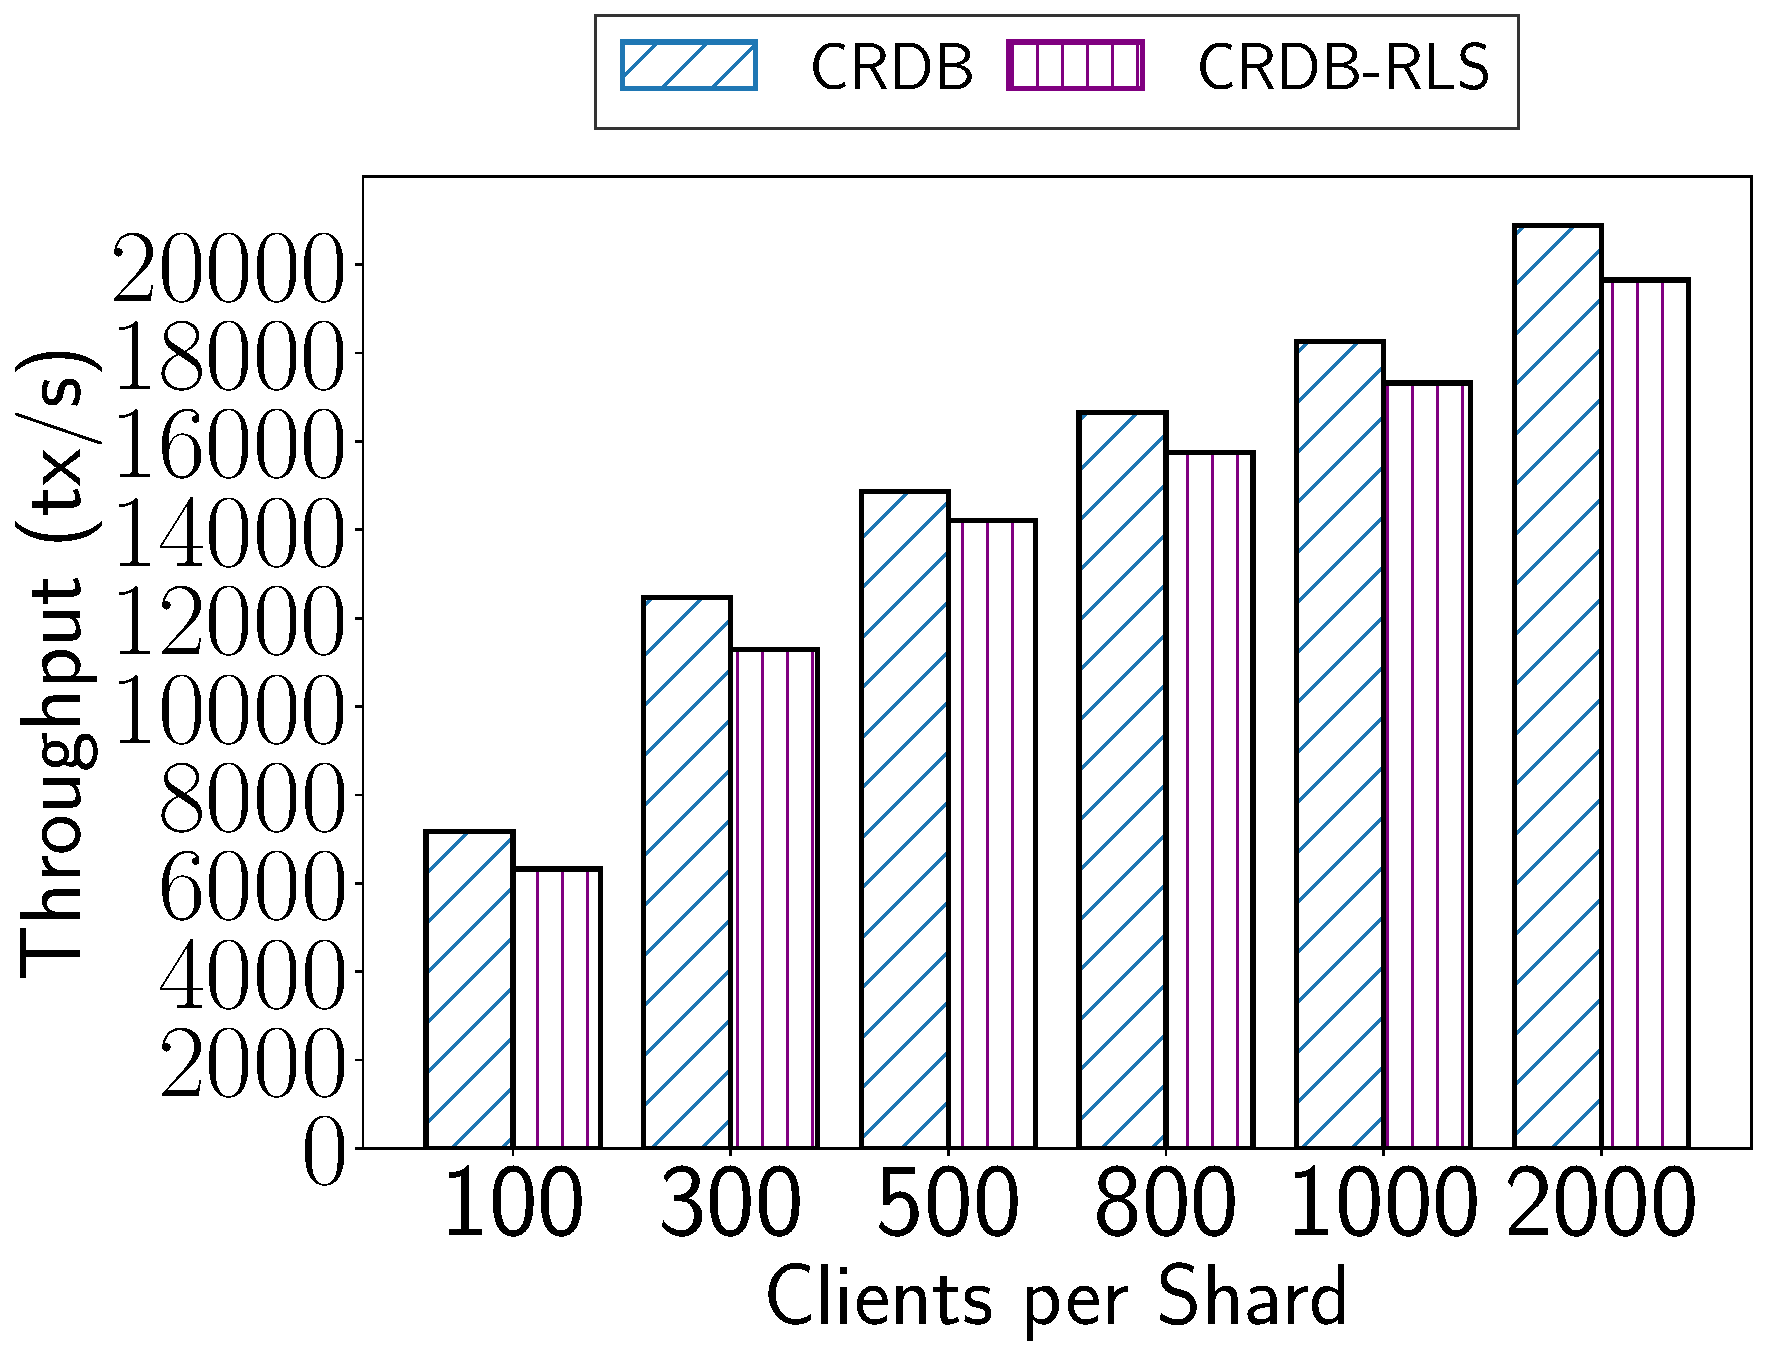
\includegraphics[width=0.49\columnwidth]{eval-figs/crdb-client--tput-kv.pdf}
	   \label{fig:eval:kv:throughput}
	}
	\subfloat[\footnotesize Overview.]{
		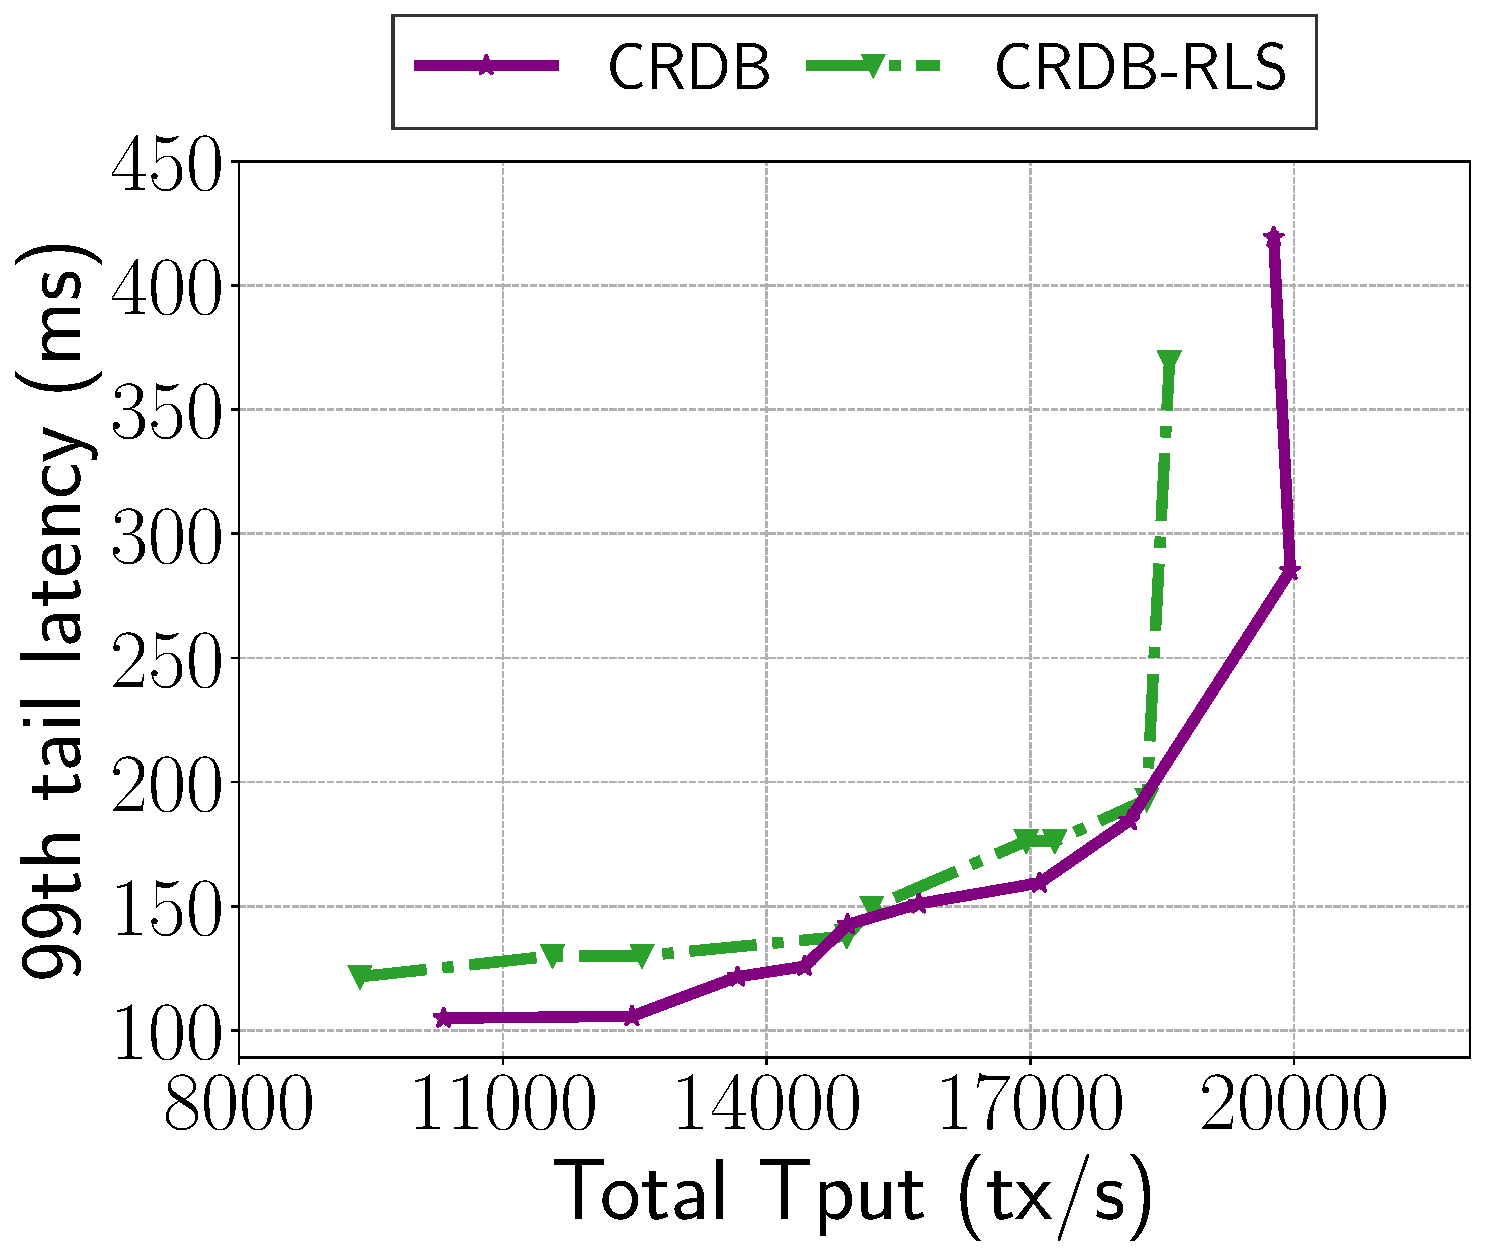
\includegraphics[width=0.49\columnwidth]{eval-figs/crdb-latency--tput-kv.pdf}
		\label{fig:eval:kv:overview}
	}
	\caption{Performance Comparison on Micro Workload.}\label{fig:eval:kv}
\end{figure}

\begin{figure}[t]
	\centering
	\subfloat[\footnotesize Throughput.]{
	   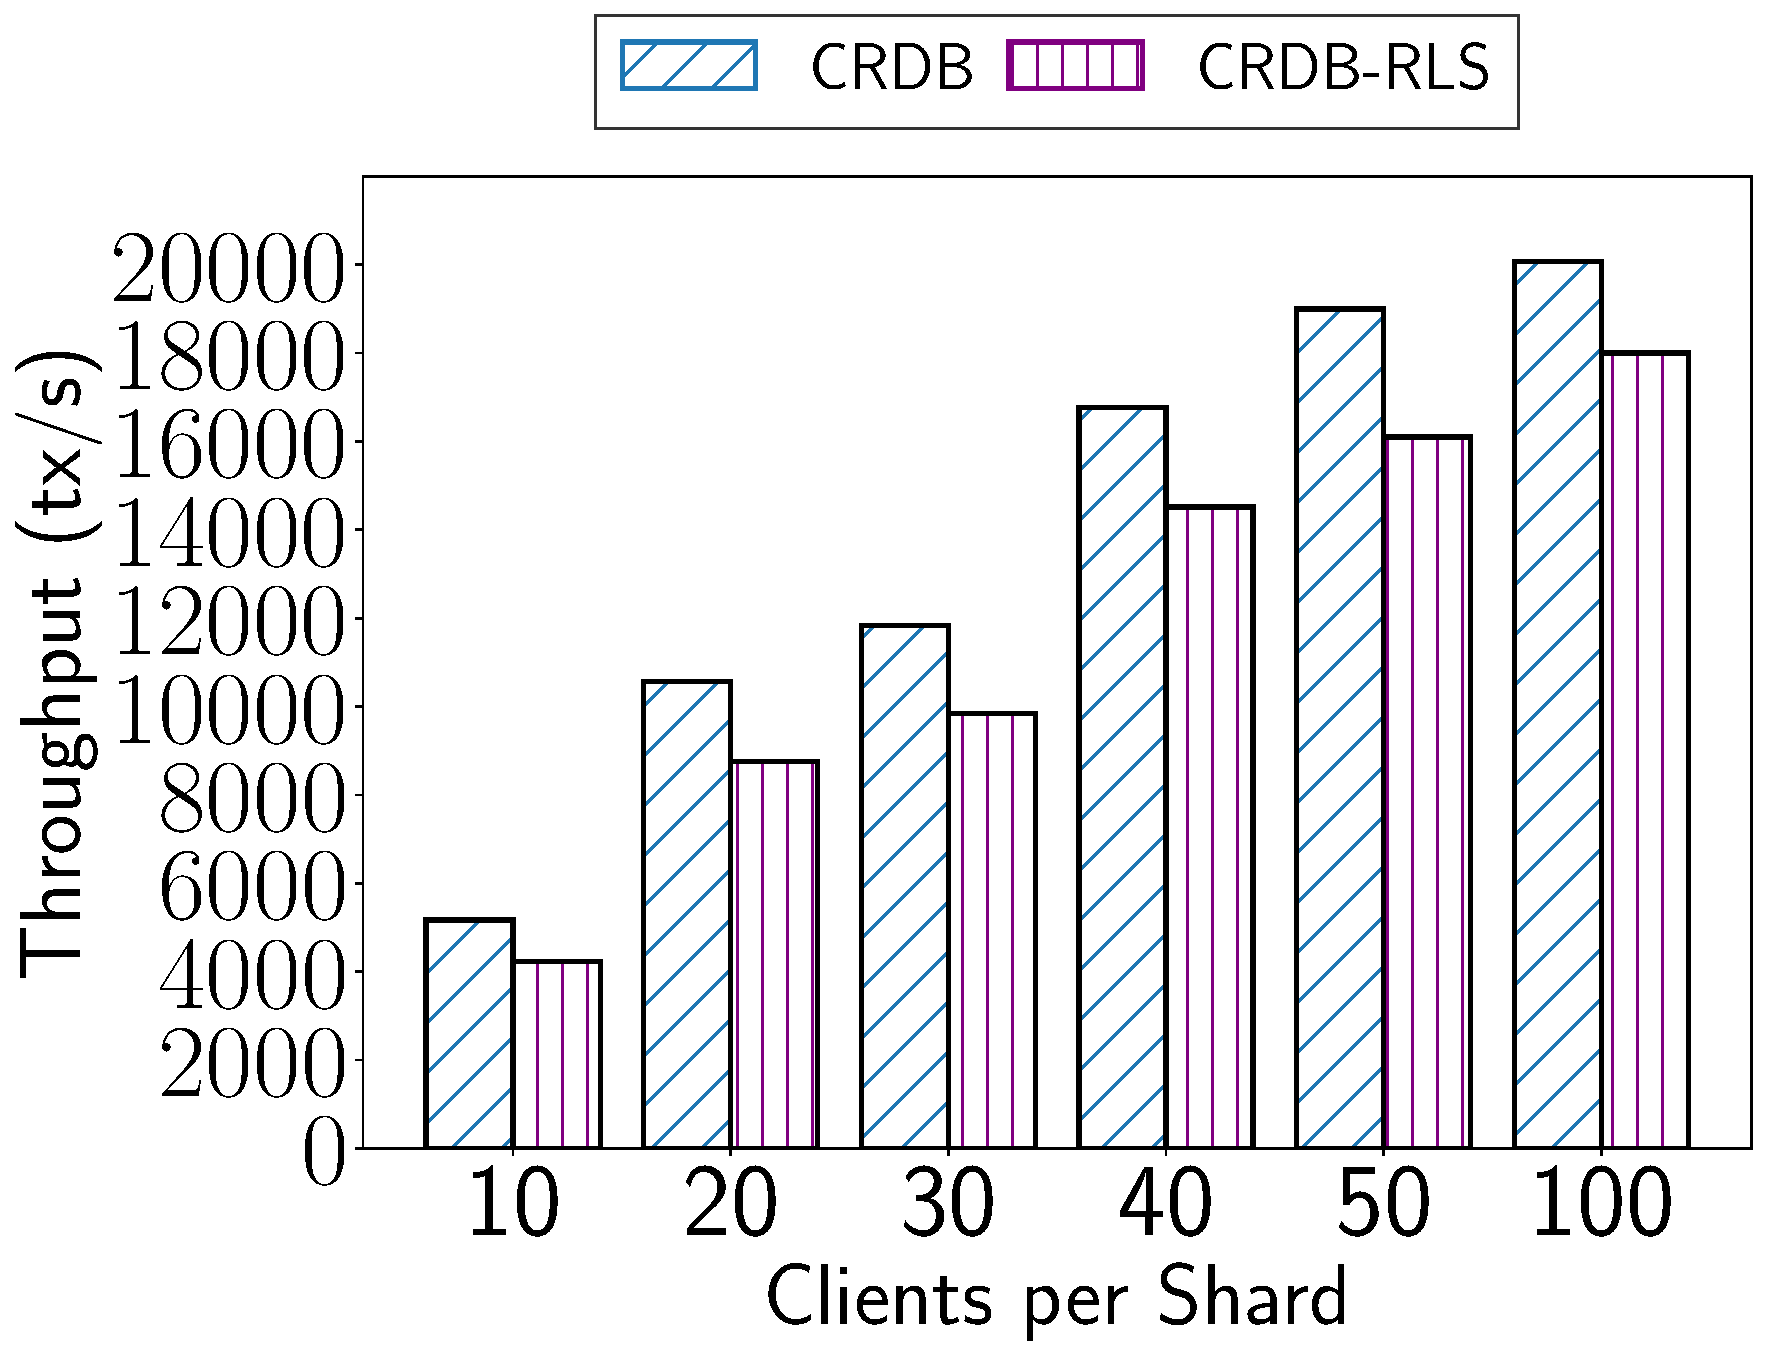
\includegraphics[width=0.49\columnwidth]{eval-figs/crdb-client--tput-ycsb.pdf}
	   \label{fig:crdb:eval:ycsb:throughput}
	}
	\subfloat[\footnotesize Overview.]{
		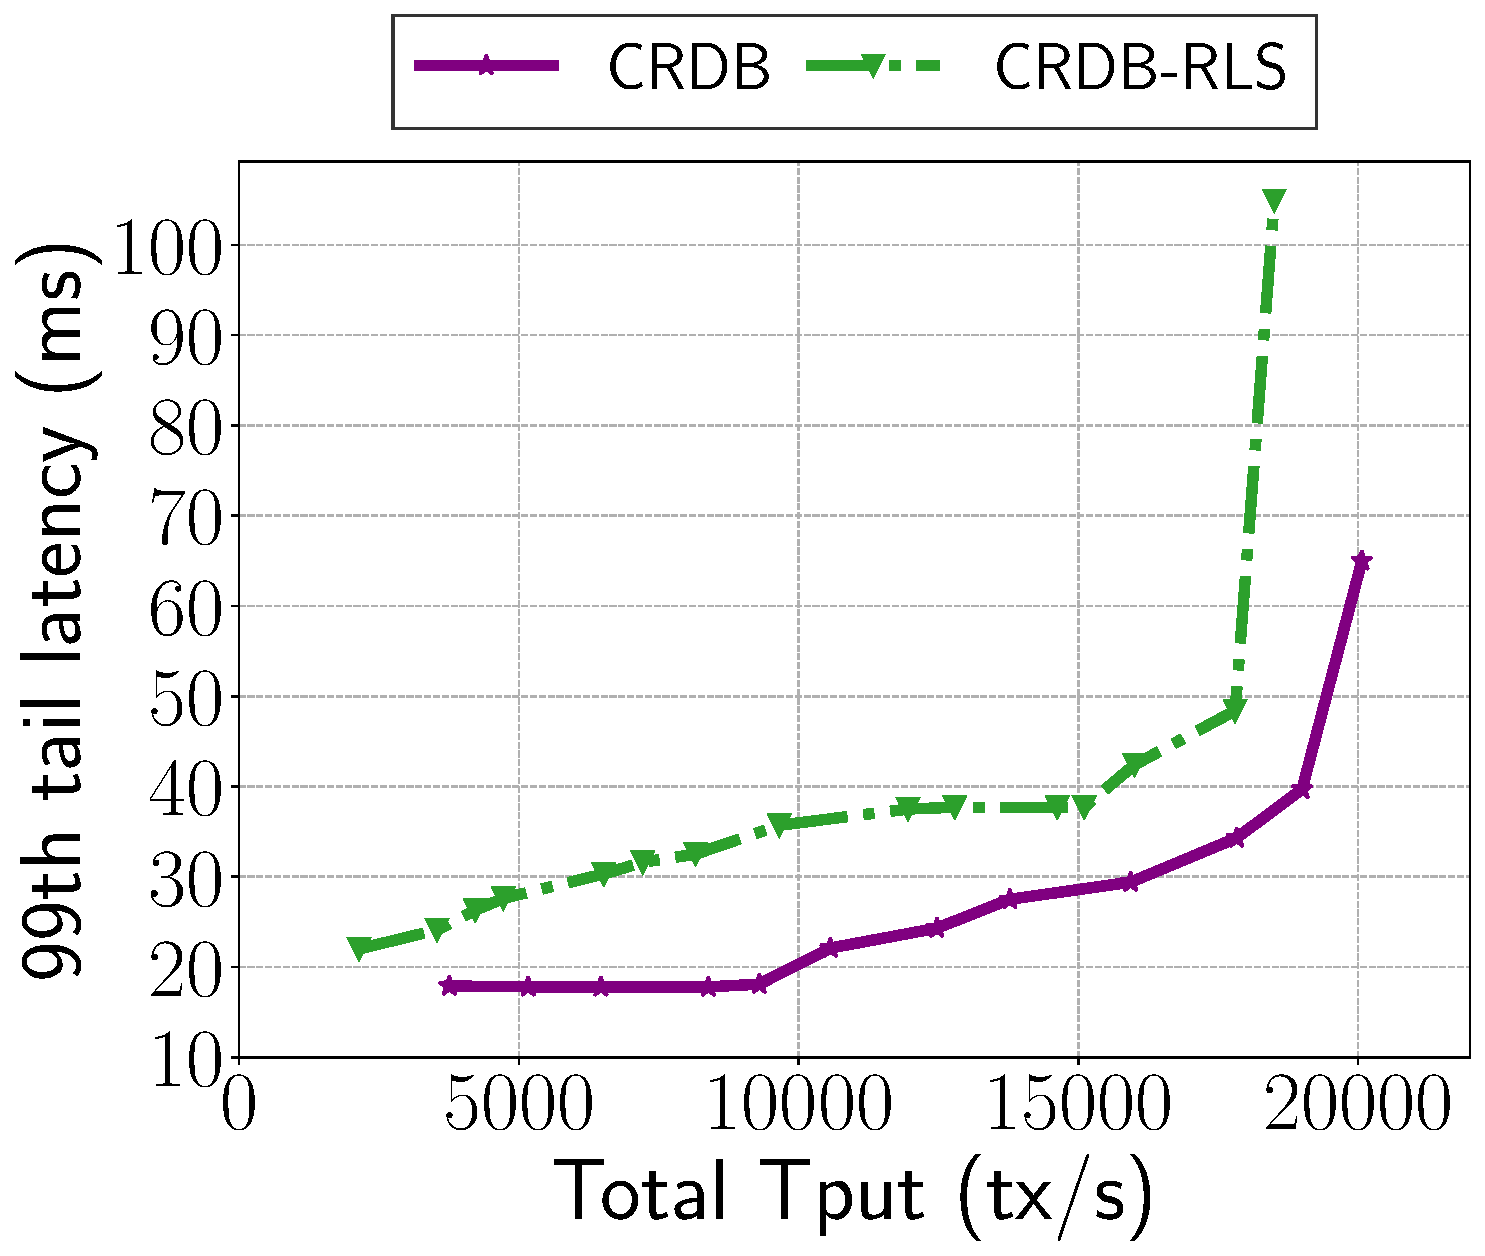
\includegraphics[width=0.49\columnwidth]{eval-figs/crdb-latency--tput-ycsb.pdf}
		\label{fig:crdb:eval:ycsb:overview}
	}
	\caption{Performance Comparison on YCSB-T (skewed).}\label{fig:crdb:eval:ycsb}
\end{figure}

Our observation of \crdbxx is that, to know whether a transaction $T_1$ may have finished before $T_2$ starts, instead of directly comparing the timestamps, a more intuitive method should be using active inquiry. In \crdb, transaction managers maintain the status of each transaction, and one can get the status of each transaction from the managers. Initially, \crdb does not adopt this active inquiry design because it can be inefficient and non-scalable to let all transactions contact a single node in a geo-distributed deployment. However, \xxcons's region-based approach enabled \crdb to record transaction states in a per-region manner (\algo{algo4}, Line 13) and enabled each transaction to inquire only relevant regions' managers (\algo{algo4}, Line 14), achieving both stronger consistency and high efficiency.

Like CRDB, CRDB-RLS allocates timestamps using hybrid-logical clocks (HLC), where physical time is
based on a node’s coarsely-synchronized system clock, and logical time is based on Lamport’s clocks. Such a mechanism benefits the design of CRDB-RLS as valid transactions can now adjust their timestamps based on logical time without frequently re-obtaining new timestamps.


\noindent\textbf{Implementations.} We implemented CRDB-RLS using the open-source codebase of CRDB with version v23.1.10 from the official sites. We modified the logic of obtaining a valid timestamp by recoding all used timestamps inside a region using sets. Our implementation is orthogonal to the optimizations introduced by its origin paper~\cite{taft2020cockroachdb} (e.g., write pipelining, parallel commits, and follower read). 

\subsection{Evaluation and Discussion} We used the same hardware and cluster setups as Spanner. For the deployments, we employed $10$ containers spanning uniformly over the machines, with each container running as a CRDB node. We used the multi-region SQL for Table partition and data replication.

\subsubsection{Performance on Micro Workload} As the configuration file of CRDB is complex and always critical to the performance, we calibrated our results by running the most basic built-in workloads provided by the CRDB codebase  (i.e., a transaction reads and writes to three keys spread uniformly across the cluster). The results are shown in \fig{fig:eval:kv}. The peak throughput of CRDB was $\sim20k$ tps, which aligns with the results shown on the official sites. Therefore, we believe our experimental results are representative. 

In addition to CRDB, we also test the performance of our implemented variation: CRDB-RLS. CRDB-RLS's peak throughput ($\sim18.6k$ tps) is slightly lower (7\%) than CRDB, while the latency is roughly the same. The slight performance degradation is caused by the higher cost of obtaining valid timestamps for IRTs.

\subsubsection{Performance on YCSB-T} We further compared the performance of CRDB and CRDB-RLS on the default YCSB-T (\chref{sec:spanner:eval}) using the calibrated configurations. The results are shown in \fig{fig:crdb:eval:ycsb}. Overall, CRDB-RLS achieved approximately $0.87\times$ to $0.91\times$ throughput compared to CRDB with various concurrencies. The peak throughput of CRDB-RLS was $12\%$ lower than CRDB, and the 99th tail latency of CRDB-RLS was $1.2\times$ to $1.6\times$ higher than CRDB.


CRDB-RLS incurred a more server performance drop on the skewed YCSB-T workloads. Compared to CRDB, CRDB-RLS may expand the contention footprint by involving more ongoing timestamps (i.e., line 16, Algorithm2). However, the overhead is still marginal, and the performance degradation is smaller than $\sim15\%$.





\subsection{Takeaways.} CRDB-RLS achieved similar performance as CRDB while providing strong consistency guarantees on real-time orders. This is because CRDB-RLS can efficiently capture ongoing transactions inside a region due to the fast networks. Recording ongoing transactions (known as transaction tables) is a common approach for processing transactions on a single machine or in a smaller cluster due to its simplicity and easy extension. We reused such an approach but with a more lightweight tracking method for ordering IRTs.

\begin{figure*}[t]
	\centering
    \subfloat[\footnotesize Allowed by \xxcons but disallowed by SS, RSS.\label{fig:rls_ss}]{
        \centering
        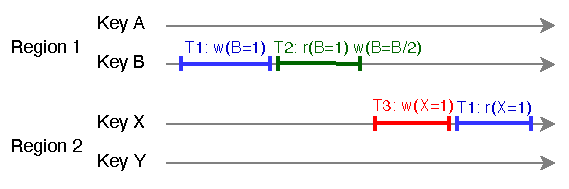
\includegraphics[width=0.63\columnwidth]{figures/RLS_SS.pdf}
    }
	\hfill
    \subfloat[\footnotesize Allowed by RSS but disallowed by \xxcons.\label{fig:rls_rss}]{
        \centering
        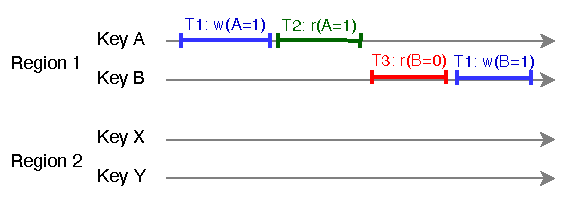
\includegraphics[width=0.63\columnwidth]{figures/RLS_RSS}
    }
    \hfill
    \subfloat[\footnotesize Allowed by \crdb but disallowed by \xxcons\label{fig:rls_crdb}]{
        \centering
         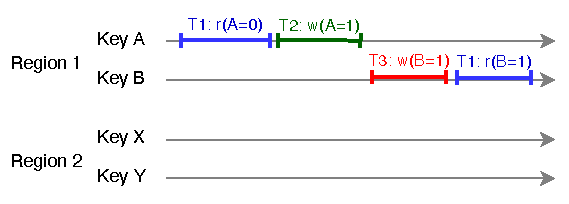
\includegraphics[width=0.63\columnwidth]{figures/RLS_CRDB.pdf}
    }
	\caption{Comparison of \xxcons with proximal levels of consistency models.}
\end{figure*}

\section{Related Works}\label{sec:related}
Transaction processing represents a well-explored area of research, with a plethora of influential works. We will provide an overview of related works in this section.

\subsection{Proximal Consistency Models}\label{sec:rls:compare}

\fig{fig:model} compares RLS to its proximal consistency models. We describe three of them in detail. All of them are serializable.

\begin{figure}[t]  
    \centering
    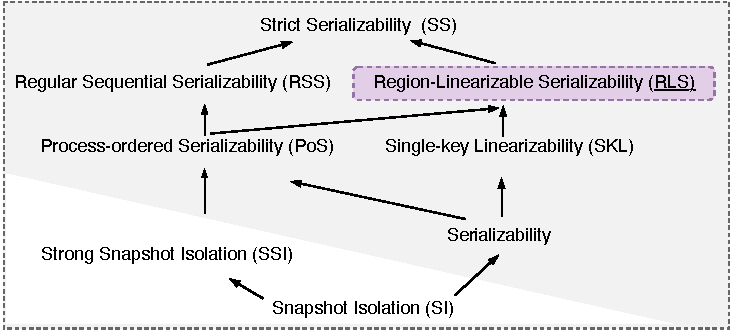
\includegraphics[width=\columnwidth]{figures/model.pdf}
  % \vspace{-5pt}
    \caption{This diagram shows how RLS compared to its proximal consistency models: SS~\cite{papadimitriou1979serializability}, RSS~\cite{rss}, SKL~\cite{taft2020cockroachdb}, PoS~\cite{daudjee2004lazy, lu2016snow}, SSI~\cite{fekete2005making}, serializability~\cite{viotti2016consistency}, and SI~\cite{anderson1998replication}. We highlight all those serializable consistency models in grey.} \label{fig:model}
  \end{figure}

\noindent\textbf{Regular Sequential Serializability (RSS)} complements \xxcons, as they focus on different aspects of distributed databases. RSS is primarily tailored for read-only transactions, permitting two read-only transactions to observe partial results of a committed read-write transaction in arbitrary orders (see our example in \fig{fig:rls_rss}). This behavior essentially violates the real-time ordering among read-only transactions.
On the contrary, \xxcons focuses on data locality within multi-region deployments, allowing a database system to relax the real-time ordering among transactions that access non-interleaved regions (refer to \fig{fig:rls_ss}). 
As illustrated in \fig{fig:rls_rss}, RSS allows transaction $T_2$ to read the writes made by a concurrent transaction $T_1$, while $T_3$ following $T_2$ reads a version preceding $T_1$. Consequently, the real-time order between $T_2$ and $T_3$ is disrupted: the real-time order between $T_2$ and $T_3$ is $T_2 \rightarrow T_3$; the serializable order enforced by RSS is $T_3 \rightarrow T_1 \rightarrow T_2$, which implies $T_3 \rightarrow T_2$.
This execution is not allowed by \xxcons since RLS ensures strict serializability (i.e., real-time order) for IRTs within the same region. 
% On the flip side, the execution shown in \fig{fig:rls_ss} is allowed by \xxcons but disallowed by RSS.

\noindent\textbf{Single-key Linearizability (SKL)} was initially proposed by CockroachDB~\cite{taft2020cockroachdb}. SKL stands as a strictly weaker variant of \xxcons. Like RLS, SKL guarantees serializability and ``no stale-reads''. However, unlike RLS, SKL does not preserve real-time orders between non-conflicting transactions. For instance, the execution illustrated in \fig{fig:rls_crdb} is permissible by SKL since there are ``no stale reads'' for each accessed key. However, it violates the real-time ordering between $T_2$ and $T_3$ in the same region, as the serial order is $T_3 \rightarrow T_1 \rightarrow T_2$, a violation not allowed by \xxcons. While weaker SKL may suffice for certain applications, other applications might necessitate stronger guarantees. Moreover, preventing consistency anomalies can significantly streamline application development.


\noindent\textbf{Process-ordered Serializability (PoS)} complements \xxcons. In a real deployment scenario, \xxcons can be stronger than PoS by associating each client with its nearby region. Specifically, PoS tracks the causal relations of each client and ensures the system preserves the ordering within each client's requests. If each client is associated with a region (e.g., sending requests to nodes within its region), \xxcons can prove to be strictly stronger than PoS since it guarantees real-time ordering for each client. 


\subsection{Transaction Priority}\label{sec:related:priority}

Compared to strict serializability (SS), one of the pivotal innovations of RLS is scheduling IRTs ahead of CRTs until the CRTs' order is established. Therefore, RLS operates under the assumption that IRTs have a higher priority than CRTs until CRTs have been ordered, after which both IRTs and CRTs are given equal priority for execution.

In this context, multi-region database developers can leverage existing transaction priority protocols to transition from SS to RLS, enhancing performance. For instance, Polaris~\cite{ye2023polaris} represents a transaction priority protocol rooted in a variant of OCC. Polaris embeds priority-related conflict detection within each record and permits priority preemption during runtime. 
Furthermore, Polaris avoids global operations, mitigating substantial overhead in a multi-region deployment. Consequently, achieving RLS should involve drawing inspiration from OCC-like concurrency control protocols. 

\subsection{Mixed Consistency Models}\label{sec:related:mixed}
Several prior works~\cite{milano2018mixt, li2012making, wang2021autogr, yang2017hierarchical, li2018fine, gao2003application, kraska2009consistency, mdcc:eurosys13} have been on manipulating weakly and strongly consistent transactions within a single database. For instance, MixT~\cite{milano2018mixt} advocates that consistency is a property of information. It proposes a new embedded language enabling users to configure the consistency guarantees for each operation manually. Similarly, Red-Blue consistency~\cite{li2012making} allows strongly and causally consistent operations to co-exist in a single system in the transaction's granularity and depends on application semantics to make ``consistency choices''. AutoGR~\cite{wang2021autogr} automatically analyzes and identifies the minimal set of the required consistency guarantees based on applications using the Z3 theorem prover. However, it relies on the application codes as inputs and only provides serializable guarantees without real-time order.

In contrast, RLS is geared towards multi-region deployments, directly integrating network semantics into the consistency model. Consequently, RLS does not depend on prior application knowledge to manually set distinct consistency guarantees for different transactions or operations. Moreover, RLS provides serializability (i.e., the strongest isolation levels) for all transactions while tailoring real-time properties to achieve heightened performance.

\section{Future Works}
The multi-region transactions set three clear objectives: high throughput, low client-perceived latency (especially for IRTs), and as strong as possible consistency. Earning all three requires careful designs to strike a balance between the three individual objectives. Our exploration of RLS opens up a new design space for achieving such goals. We draw some lessons worth further research:

\begin{itemize}[leftmargin=*, itemsep=1pt]
\setlength{\parsep}{0pt}
\setlength{\parskip}{0pt}
\setlength{\parindent}{1em}
    \item \textbf{Multi-Layered Consistency Model.} Modern network exhibits a multi-layered structure~\cite{zhang2023redt, webb2011topology}. For instance, Cloud providers (e.g., Huawei~\cite{huawei:region}) are diligent in using CXL- and RDMA-based networks inside a data center, a dedicated network between data centers inside a region, and public networks across the regions. In this work, we have explored the consistency model for multi-region deployment by treating IRTs and CRTs differently. However, a more fine-grained design may still be desirable to tightly fit consistency guarantees into the network stack. For instance, in-network ordering technologies~\cite{bidl:sosp21, epaxos:sosp13, li20211pipe, choi2023hydra}, which leverage the properties of the network for order, are proposed for in-data center deployment. How to combine such technologies with geo-distributed transactions is still an open problem. A multi-layered consistency model may work as the glue to bridge the design of in-network transaction processing technologies with geo-distributed transaction processing technologies.
    \item \textbf{Data Locality and Partial Replication.} Even though RLS provides practical mitigation for achieving high throughput and low latency for both CRTs and IRTs, the cost of remote reads cannot be fundamentally removed. Therefore, an efficient data partition and replication policy are still critical for real-world usage: a good partition policy~\cite{abebe2020dynamast, abebe2020morphosys, curino2010schism, pavlo2012skew, zamanian2015locality} can vastly reduce the ratio of remote reads, and a cautious replication policy~\cite{taft2020cockroachdb, dast:eurosys21, schiper2010p} can balance the overhead of data synchronization and remote access. 
\end{itemize}

\vspace{10pt}
\section{Conclusion}\label{sec:conclusion}
This work uncovered fundamental bottlenecks in strictly serializable concurrency control algorithms used in multi-region deployments. As the consistency model inherently enforces these bottlenecks, many proposals turn to lift the restrictions by adopting weaker consistency. However, we found that all existing consistency models are inadequately designed for multi-region deployments: they are either overly stringent or have room for improvement without incurring significant performance penalties. 

In response, we propose Region-Linearizable Serializability (RLS), the first consistency model meticulously tailored for multi-region deployment. Following the RLS methodology, we design, implement, and evaluate two practical system variations based on open-sourced codebases: Spanner-RLS and CRDB-RLS. The code of our stereotypes is available at {\color{darkred}{\url{https://github.com/vldb24p771/spanner_rls}}} and {\color{darkred}{\url{https://github.com/vldb24p771/crdb_rls}}}, respectively. 

Our evaluation results demonstrate that RLS can significantly enhance the performance of Spanner (i.e., from $1.16\times$ to $89.01\times$ higher throughput) and further strengthen the consistency guarantees of CRDB without significant performance drop (i.e.,  $<15\%$). 

\clearpage


\bibliographystyle{IEEEtran}
\bibliography{bib/database,bib/biblio,bib/blockchain,bib/edge,bib/htap}
\end{document}
